\documentclass[letterpaper,oneside,12pt,spanish]{book}

\usepackage[utf8]{inputenc}
\usepackage[spanish]{babel}
\usepackage[T1]{fontenc}
\usepackage{tocbibind} % Bibliografía en el indice
\usepackage{titlesec} % Posibilidad de editar los formatos de chapter
\usepackage{amsmath,amssymb,mathrsfs} % Matemáticas varias
\usepackage{hyperref} %Esto te hace un pequeño esquemita al lado
\usepackage{listings}
\usepackage{anysize} 
\usepackage{algorithmic} % Para pseudocódigo de algoritmos
\usepackage{algorithm}
\usepackage{appendix} % Para tener apéndice en vez de capítulos
\usepackage{verbatim}
\usepackage{multirow}
\usepackage{array}
\usepackage{pdflscape}



% --- Arreglos varios para la inclusion de imagenes
\usepackage[pdftex]{graphicx}
\usepackage{subfigure}
\usepackage{graphicx}
\usepackage[usenames,dvipsnames]{color}
\DeclareGraphicsExtensions{.png,.jpg,.pdf,.mps,.gif,.bmp}

% --- Para las dimensiones de los márgenes etc
% \frenchspacing \addtolength{\hoffset}{-1.5cm}
% \addtolength{\textwidth}{3cm} \addtolength{\voffset}{-2.5cm}
% \addtolength{\textheight}{4cm}
\marginsize{3.8cm}{2.5cm}{2cm}{2cm} 

\setlength{\parskip}{0.7em}

% --- Para el encabezado
\usepackage{fancyhdr}
\fancyhead[R]{UTFSM}\fancyhead[L]{} \fancyfoot[C]{\thepage}
\pagestyle{fancy}

% --- Para las tablas
\renewcommand{\tablename}{Tabla}
\renewcommand{\listtablename}{Índice de tablas}

% --- Para los apendices
\renewcommand{\appendixname}{Anexos}
%\renewcommand{\appendixtocname}{Anexos}
%\renewcommand{\appendixpagename}{Anexos}
% -------------------------------------------------------- %

\title{•}
\author{Paulina Andrea Silva Ghio}

\lstset{ %
language=C,                % choose the language of the code
basicstyle=\footnotesize,       % the size of the fonts that are used for the code
numbers=left,                   % where to put the line-numbers
numberstyle=\footnotesize,      % the size of the fonts that are used for the line-numbers
stepnumber=0,                   % the step between two line-numbers. If it's 1 each line 
                                % will be numbered
numbersep=5pt,                  % how far the line-numbers are from the code
backgroundcolor=\color{white},  % choose the background color. You must add \usepackage{color}
showspaces=false,               % show spaces adding particular underscores
showstringspaces=false,         % underline spaces within strings
showtabs=false,                 % show tabs within strings adding particular underscores
frame=single,	                % adds a frame around the code
tabsize=2,	                % sets default tabsize to 2 spaces
captionpos=b,                   % sets the caption-position to bottom
breaklines=true,                % sets automatic line breaking
breakatwhitespace=false,        % sets if automatic breaks should only happen at whitespace
title=\lstname,                 % show the filename of files included with \lstinputlisting;
                                % also try caption instead of title
escapeinside={\%*}{*)},         % if you want to add a comment within your code
morekeywords={*,...}            % if you want to add more keywords to the set
}

\begin{document}
\frontmatter
\begin{titlepage}

\begin{center}

\textsc{\Large Universidad Técnica Federico Santa María}\\
\textsc{\large Departamento de Informática}\\
\textsc{\large Valparaíso, Chile}\\[1.5cm]

% Upper part of the page

\includegraphics[width=0.3\textwidth]{figures/utfsm.jpg}\\[1cm]    

% Title
{ \huge Una Arquitectura de Referencia para Web Browsers, como Unificación de Conceptos de Amenazas y Defensas Asociados }\\[2cm]

% Author and supervisor
\text{\Large Paulina Andrea Silva Ghio}\\[2cm]
\text{\large Memoria para obtar al título de: Ingeniera Civil Informática}\\[3cm]
\text{\large Profesor Guía: Raúl Monges}\\
\text{\large Profesor Correferente: Javier Cañas}

\vfill

% Bottom of the page
{\large \today}

\end{center}

\end{titlepage}
 
%\begin{flushright}  
\null \vspace{\stretch{1}}
\emph{Si sta come \\d'autunno \\sugli alberi \\le foglie \\ \textbf{Soldati} di Guiseppe Ungaretti (1918)} 
\end{flushright}
\newpage 
%\chapter*{Agradecimientos}
\label{chap:agrad}

Con esta Memoria voy a dar por finalizado los largos 6 años de la carrera, que terminaron por ser casí 7 y algo más por el Magister. No me arrepiento de mis decisiones en la parte académica, pero a veces en lo personal creo que pudo haber sido de otra manera. Tuve muchos desafíos que realizar al estudiar para este trabajo, partiendo por mi nulo conocimiento en Seguridad y a veces la falta de motivación. Sin embargo, estoy acá en este momento gracias a esas decisiones y experiencias que he ganado en el intertanto. Gracias a todas las personas que me motivaron, en especial, a mi profesor guía Raúl Monge (UTFSM) y el profesor Eduardo Fernandez (Florida Atlantic University), quienes me mostraron un camino interesante a seguir.

Quiero agradecer a todos mis amigos de la Universidad, que son muchos, y aquellos que la abandonaron por un camino mejor o más interesante. Gracias por haberse presentado en mi vida y hacerla entretenida. Sin la risa y diversión en mi vida, probablemente sería una persona amargada. Gracias a todos por soportar mi malhumor y comprenderme cuando estoy angustiada. Gracias también por haberme ayudado academicamente, que si bien todos creen que soy matea nada tengo de eso; solo estudio demasiado y a veces no de la mejor manera.

Gracias Mamá y Papá por darme educación. Se que no es fácil pagar tanto dinero todos los meses, pero en verdad se los agradezco siempre. Gracias a que he tenido la oportunidad de estudiar en una Universidad, se cuán importante es la educación y que debo aprovecharla al máximo. Se que muchas veces tuvimos varios problemas mientras yo crecía, pero quiero hacerles saber que estoy agradecida de ser su hija. Gracias por cuidar y confiar en mi.

Gracias Panchomon por todo, eres una existencia muy importante en mi vida y espero que lo sepas. Gracias Micchan, por ser mi manta cuando estoy triste. Ustedes dos han sido los pilares más grandes que he tenido en estos años de universidad. Gracias Fernando, Samuel, José Miguel, Francisco, Matías y Andrés, por ser mis \textit{dudes} y soportarme siempre. Gracias Priscilla, Scarlet y Susana, por ser mis amigas más cercanas en la Universidad. Ko-chan, Yurie, Asumi, Geso y Motoki a ustedes también gracias por apoyarme siempre. Finalmente, ¡gracias a todos!, por tenerme una gran paciencia a lo largo de estos años, por levantarme el ánimo cuando no quiero dar más pasos hacia adelante, por inspirarme a ser mejor, y por estar en mi vida de alguna que otra forma. También muchas gracias al que lee este documento, en especial, por darse el tiempo de hacerlo. 
\newpage 
% Resumen a grandes rasgos de lo existente (resumen del estado del arte y resumen del trabajo realizado)

\section*{Resumen}
\label{chap:resumen}

El Web Browser es una de las aplicaciones más usadas - \textit{killer app} - y también una de las primeras en aparecer en cuanto se creó el Internet (Década de los 90). Por lo mismo, su nivel de madurez con respecto a otros desarrollos es significativo y permite asegurar ciertos niveles de confianza cuando otros usan un Web Browser como cliente para sus Sistemas. 

Actualmente muchos desarrollos de software crean sistemas que están conectados a la Internet, pues permite agregar funcionalidades al sistema y facilidades para sus \textit{Stakeholders}. Esto lleva a depender de un cliente web, cómo un \textit{Web Browser} que permita el acceso a los servicios, datos u operaciones que el sistema entrega. Sin embargo, la Internet influye en la superficie de ataque del nuevo sistema que se implementó, y lamentablemente tanto Stakeholders como muchos desarrolladores no están al tanto de los riesgos a los que se enfrentan.

En esta Memoria presentada al Departamento de Informática (DI) de la UTFSM\footnote{Universidad Técnica Federico Santa María} Casa Central, se al incursionará en el ámbito de la seguridad del Web Browser, con el objetivo de obtener documentos formales que servirán como herramientas a personas que Desarrollen Software y hagan un fuerte uso del Navegador para las actividades del sistema desarrollado.

\section*{Abstract}

The Web Browser is known as one of the most used applications - or \textit{killer app} - and also was the first introduced when the Internet was created (1990). Which is why, it's significant maturity level is above in comparison with other developements and can assure a certain level of \textit{trust} whenever it is used as a client with other systems.

\label{chap:abstract}


 
\markboth{}{}
\newpage
\tableofcontents 
\newpage
\listoffigures
\newpage
\listoftables
\newpage	
\renewcommand{\sectionmark}[1]{\markright{\thesection\ #1}}

\mainmatter

%Intro CHECKED!!


\chapter{Introducción}
\label{chap1:intro}


\section{Contexto General}
\label{chap1:CG}

Entre 1989 y 1990, Tim Berners-Lee acuñó el concepto de \textit{World Wide Web} y con ésto realizó la construcción del primer \textit{Web Server}, \textit{Web Browser} y las primeras páginas \textit{Web}. Mucho antes que aparecieran los grandes sistemas que ahora conocemos, el \textit{Web Browser} permitía navegar páginas estáticas y realizar una serie de acciones limitadas a las tecnologías de ese tiempo. En la actualidad el \textit{browser} es la herramienta predilecta por todos, desde comprar tickets para una película, realizar reuniones por videoconferencia y muchas otras tareas que invitan a nuevas formas de interactuar y comunicar.

Durante la conocida \textit{guerra de navegadores}, en la decada de los noventa, los \textit{browser} tuvieron solo el objetivo de poder adquitir la mayor cantidad de usuarios posibles, entregando mejores funcionalidades que sus competidores. Debido a esto era habitual encontrar muchos parches que solucionaban problemas de seguridad, dada la cantidad de errores de programación y casi nula estructura del navegador, dado que no había una pronta preocupación por el diseño. Además la nula documentación que existía debido a la gran competitividad, muchas veces hacía que las extensiones hechas por \textit{third-parties} creaban más agujeros de seguridad, que nuevas funcionalidades. El inicio del Software Libre u \textit{Open Source}, cambió el escenario y las circunstancias pero aún así, existen navegadores propietarios que no exponen la arquitectura de sus aplicaciones.

En el último tiempo el mercado de los \textit{Web Browser} ha crecido bastante (Figura \ref{fig:UsageShare}), principalmente debido a la robustez que éstos poseen y a la cantidad de años que llevan desarrollándose en la industria del Desarrollo de Software. Los navegadores más conocidos son: Google Chrome o su versión Open Source Chromium, Firefox, Internet Explorer, Opera y Safari; siendo los primeros 3 el enfoque de este trabajo.

    \begin{figure}[h]
        \centering
        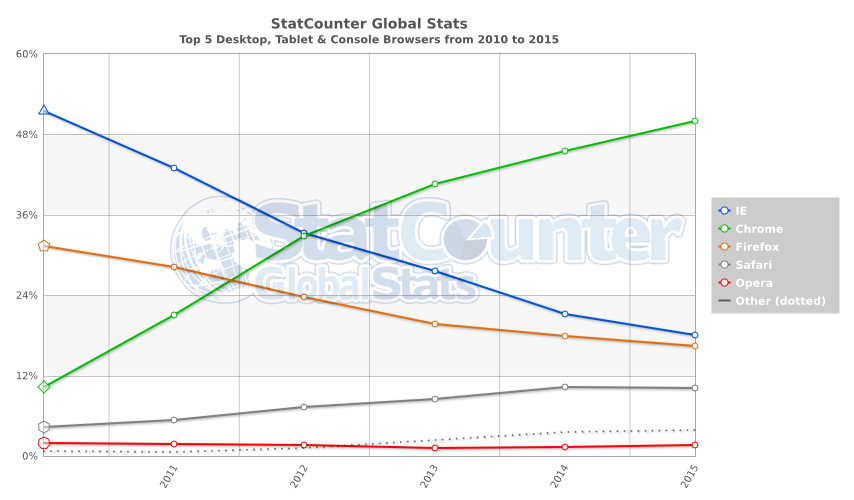
\includegraphics[width=1\textwidth]{figures/StatCounter-browser-ww-yearly-2010-2015.png}
        \caption{Porcentaje de uso de Navegadores. Fuente: \cite{statBrow}}
        \label{fig:UsageShare}
    \end{figure}

La \textit{Web 2.0} se inició con el uso intensivo de tecnologías como AJAX, y ésto ha permitido una nueva simbiosis entre el usuario, el Web Browser y el Servidor o Web Server que se comunican entre sí. El Navegador Web es una herramienta indispensable para todo tipo de tareas computacionales como comunicacionales, su existencia a penetrado completamente en las labores diarias de todos nosotros. En este mismo instante, la Web a evolucionado nuevamente obteniendo un nuevo nombre: \textit{Web 3.0}, donde se realiza el uso de inteligencia artificial y sistemas de recomendación para generar nuevos tipos de contenido para el usuario.


\section{El Problema: Desarrollo de Software y Seguridad}
\label{chap1:SD_SS}

Ningún Desarrollo de Software es igual al anterior. Por cada nuevo proyecto que surge es necesario ver qué tipo de proceso es el que se usará, qué personas serán parte del grupo de trabajo, qué condiciones económicas estará expuesto, qué \textit{Stakeholder} están pendientes de que el Proyecto salga exitoso y un sin numero de variables, no menos importantes a considerar. Por lo tanto dependiendo de lo anterior, los sistemas podrían llegar a ser simples o muy complejos. En consecuencia, se hace necesario tener ciertas metodologías que aseguren que se cumplan con todos los Requerimientos Funcionales como No-Funcionales del Sistema a construir. Sin embargo un problema que existe recurrentemente, es que la mayoría del Software construído contiene numerosos \textbf{defectos} y \textbf{errores}, generando así \textbf{vulnerabilidades} que son encontradas y explotadas por los atacantes, generando un compromiso parcial o total del sistema \cite{goertzel2007software}. Lo anterior sucede frecuentemente por que los sistemas no son desarrollados teniendo en cuenta la seguridad \cite{Yoder1998, fernandez2004methodology, WhyteHarrison}.

Muchas veces al desarrollar sistemas, se prefiere utilizar API's\footnote{Application Programming Interface} de otros sistemas para poder incluir funcionalidades ya implementadas, fomentando así el Reuso de piezas de Software. Si bien lo anterior es una buena práctica, si el sistema no cuenta con las medidas de seguridad necesarias, estas piezas podrían ser causa de amenazas de seguridad que terminarían por corromper el sistema y en consecuencia podría causar una pérdida monetaria a los \textit{Stakeholders}. Lo expuesto anteriormente ejemplifica perfectamente lo que tienen que lidiar los equipos de trabajo en proyectos de Desarrollo de Software, cuando dentro de sus preocupaciones la seguridad queda como un trabajo extra y no como parte del desarrollo completo. 

Bien es sabido que un proyecto en producción que presente problemas que involucren a varias entidades, el costo asociado puede llegar a ser altísimo \cite{cert}, sin olvidar que podría llegar a afectar la Confidencialidad, Integridad y Disponibilidad de los datos de los involucrados con el sistema  \cite{interCoursera}. Por esto mismo, es imperante que sean entendidos, desde el comienzo, los \textit{concerns} de los \textit{Stakeholders} y los Requerimientos de Seguridad asociados, y que adémás todos los involucrados los entiendan perfectamente. Según \cite{WhyteHarrison} la falta de preocupación en temas de seguridad en desarrollos de software no tiene una raíz principal, diversos factores como: la falta de estudios de seguridad en las mallas curriculares de las Universidades, pocos fondos para la investigación, la falta de iniciativa y precoupación desde la industria, el exceso de confianza de los desarrolladores, etc., son los causantes de las futuras vulneraciones en sistemas críticos. 

La literatura que habla de la construcción de \textit{Secure Software} o Software Seguro, indica que los practicantes de Desarrollo de Software deben entender, en gran medida, los problemas de seguridad que podrían llegar a ocurrir en sus sistemas. No basta con saber como unir las piezas, no basta con que cada pieza de por si sea segura, si los componentes del sistema no actuan de forma coordinada probablemente éste no será seguro \cite{fernandez2013security}, dado que la seguridad es una Propiedad Sistémica que necesita ser vista de manera holística y al inicio del proceso.

Un sistema cualquiera conectado al internet y accesado por un usuario a través de un Navegador, estará en algún momento de su vida útil bajo amenazas que el Desarrollador debe estar al tanto. Al conocer los peligros es posible comunicar a los \textit{Stakeholders}, de los posibles peligros a los que se enfrentan, aún cuando en el equipo de Desarrolladores no exista un experto en seguridad. Bajo esta misma lupa, una Arquitectura de Referencia permitiría comunicar efectivamente los componentes, interacciones y comportamientos existentes entre el \textit{browser} y el sistema con el que se comunica, de tal manera que sería posible entender los posibles problemas que el \textit{Browser} puede llegar a generar. 

\section{Motivación: ¿Por qué estudiar el Browser?}
\label{chap1:motiv}

Con la aparición de la \textit{Web 2.0 y 3.0}, con el uso de \textit{AJAX}, inteligencia artificial y sistemas de recomendación, permitieron nuevas formas de interacción entre usuarios y sistemas, lo que causó que el \textit{browser} fuera usado extensivamente en los nuevos Desarrollos de Software dado que:
\begin{itemize}
	\item Permite disminuir los costos de construir un programa Cliente (desde cero) para el usuario del sistema.
	\item Actualmente la Seguridad implementada en los \textit{Web Browser} es bastante buena, dado que existen grandes compañias se aseguran de ello (Google, Microsft, Mozilla entre las más conocidas). 
	\item El \textit{browser} es una herramienta indispensable. La mayoría de los sistemas que lo usan en la vida cotidiana son de tipo: \textit{online banking}, declaración de impuestos, promoción de empresas o tiendas, compras, y mucho más.
\end{itemize}

Sin embargo los sistemas que dependen del uso del \textit{Browser}, deben de tener en cuenta las posibles amenazas de seguridad a las que se enfrentarán por el solo hecho de usarlo. Para un proyecto de gran envergadura, sería un error no tener en consideración los posibles peligros que trae el uso del \textit{Browser}, y es el deber de todo integrante del equipo de Desarrollo tener el conocimiento de la seguridad del Cliente Web. El entendimiento de la estructura subyacente del Web Browser podría asegurar que las personas que trabajen en el desarrollo, comprendan los \textit{trade-off} al momento de diseñar un Software que necesite la colaboración del Navegador Web \cite{535061, 2005-grosskurth-browser-refarch,preprint-grosskurth-browser-archevol}; poniéndolo de otra forma, un atacante es capaz de explotar un ataque en el sistema, dado que tiene el conocimiento subyacente del \textit{Browser}, conoce sus vulnerabilidades y mecanismos de defensa.

En \cite{goertzel2007software, WhyteHarrison} mencionan que la cantidad de tiempo dedicado en temas de seguridad, por los estudiantes en áreas de la Información/Computación/Software es casi nula. Si bien existen diversos factores \cite{WhyteHarrison} que pueden ser causa de este comportamientos, principalmente las universidades y las industrias son un fuerte factor en la adopción de un cambio de mentalidad. Desarrollar un sistema crítico (o no) pero seguro, representa un gran desafío. No solo para los desarrolladores, si no también para los involucrados indirectamente, como los usuarios que navegan por el \textit{browser} para hacer uso de éste sistema. Por lo mismo, es entendible que la seguridad sea un tema complicado de impartir, pero eso no significa que sea imposible. Nuestro trabajo tiene la intención de presentar un trabajo conceptual, que permita entender más este atributo de calidad y que pueda ser ayudar a otros desarrollos ser más seguros.

Este trabajo tiene una motivación principal. Ésta es ayudar a quién lo necesite con el conocimiento necesario para entender el funcionamiento y construcción del Cliente, el Web Browser, los beneficios detrás de la Seguridad implementada en el \textit{Browser} y de los peligros existentes de los que nos protegen. De esta manera se espera que alguien que lea este trabajo, tanto Estudiantes como Desarrolladores de Softwares, obtengan el conocimiento necesario al momento de trabajar junto con el Navegador Web al realizar un Desarrollo de Software que dependa de éste.

De nuestro conocimiento hasta el momento, no existe ninguna propuesta de Arquitectura de Referencia del \textit{Browser} moderno, solo existe material desactualizado que no se adecua al paisaje actual \cite{2005-grosskurth-browser-refarch}. Creemos que una falta de conocimientos de seguridad con respecto al \textit{Browser}, podría afectar de forma directa el desarrollo de aplicaciones que lo utilizan. Por esto mismo, una guía o compilado de información, semi-formal, que una los conceptos y componentes, como lo hace una Arquitectura de Referencia, podría enseñar a desarrolladores no expertos en seguridad, los peligros que existen. Nuestro trabajo explaya a la seguridad como una propiedad sistémica que debe ser tomada en cuenta desde el inicio del sistema \cite{fernandez2004methodology, fernandez2006defining, braz2008eliciting, fernandez2013security, Fernandez2011}.


\section{Contribuciones}
\label{chap1:contr}

Dada la falta de documentación para enseñar a desarrolladores no expertos en seguridad, acerca de los componentes, interacciones y comportamientos del Web Browser, el \textbf{Objetivo General} de esta Memoria es: 
\begin{center}
	Generar un cuerpo organizado de información sobre el Web Browser y su Seguridad, de tal manera que se pueda sistematizar, organizar y clasificar el conocimiento adquirido en un documento, con formato semi-formal, tanto para Profesionales como Estudiantes del área Informática que estén insertos en el área de Desarrollo de Software.
\end{center} 

Este trabajo busca cumplir con los siguientes Objetivos Específicos:

\begin{itemize}
	\item Comprender los conceptos relacionados al navegador web, sus componentes, interacciones o formas de comunicación, amenazas y ataques a los que puede estar sometido, como los también los mecanismos de defensa. Esto se realizará a través de un Estado del Arte sobre el Browser.
	\item Identificar actores, componentes, funciones, relaciones, requerimientos y restricciones del Navegador, para lograr abstraer una Arquitectura de Referencia (AR) a partir de documentación disponible en internet, blogs de desarrolladores, papers e iniciar un pequeño catálogo de Patrones de Mal Uso. Esto permitirá condensar el conocimiento obtenido en el punto anterior a través de documentos semi-formales, lo que permitirá generar una guía para comunicar los conceptos relevantes que pudieran afectar la relación existente entre un desarrollo de software y el navegador.
	\item Profundizar el conocimiento en ataques relacionados con métodos de Ingeniería Social.
	
\end{itemize} 

Particularmente se ha escogido como metodología base la dada por \cite{braz2008eliciting,fernandez2013security}. Una Architectura de Referencia (AR) tiene como objetivo el mismo descrito en \cite{2005-grosskurth-browser-refarch, preprint-grosskurth-browser-archevol, Avgeriou2003, Galster2011a}, éste es capturar la esencia de la arquitectura a través de una colección de sistemas similares, por medio del reuso arquitectónico, y además ayudar a los \textit{implementors} o desarrolladores del software, a entender los \textit{trade-off} cuando se diseñan nuevos sistemas, y puede ayudar a los mantenedores de estos sistemas a entender el código \textit{legacy} detrás los navegadores que trabajan a mano a mano. Una Arquitectura de Referencia permite además comparar las diferencias en decisiones de diseño del Navegador y así poder entender los cambios realizados a lo largo del Desarrollo de un sistema. Junto con lo anterior, ĺa AR permitirá tener una visión holística del sistema y mostrará las decisiones de alto nivel para asegurar la Seguridad del sistema. 

Por otra parte, los Patrones de Mal Uso o Uso Indebido, permitirán enseñar y comunicar las posibles formas en que tal sistema puede ser usado inapropiadamente.

En este trabajo se presentará nuestra Arquitectura de Referencia y un Patrones de Uso Indebido, que usarán la AR contruída para mostrar los componentes y mensajes que una amenaza puede realizar, con tal de lograr un ataque en el \textit{Browser}. El uso de patrones nos permitirá abstraer compontentes y comunicaciones entre dichos sistemas, al mismo tiempo que vislumbrará los mecanismos de seguridad implementados. Los patrones son herramientas de gran valor, que permiten generar el entendimiento de los aspectos funcionales y pueden complementar con otros patrones relacionados para alcanzar una arquitectura más entendible. Estos patrones serán presentados usando el template POSA \cite{buschman1996system} y UML, para así modelar las interacciones entre los diversos componentes de la arquitectura.

\section{Metodología}
\label{chap1:Met}
Este trabajo se realizará de la siguiente forma:
\begin{enumerate}
	\item Introducción de un \textit{Framework conceptual} para entender los conceptos relacionados.
	\item Hablar sobre los las (in)seguridad en el Browser, a través de los posibles ataques que se pueden dar en el Browser y como éstos pueden afectar a los sistemas que lo usan.
	\item Contruir un Estado del Arte sobre el \textit{Browser}, sobre las distintas arquitecturas, lo que se ha hecho en Arquitecturas de Referencia en el Browser, o patrones relacionados a éste.
	\item Identificar los conceptos, actores, componentes, interacciones y funciones, para poder generar una Arquitectura de Referncia del Browser.Con esto se construirá patrones de arquitectura que definan los componentes y responsabilidades.
	\item Contruir patrones de Mal Uso/Uso Indebido por medio del punto anterior.
\end{enumerate}

\section{Estructura del Documento}
\label{chap1:estruct}

El presente documento trata del trabajo de Memoria que se divide en las siguientes partes:

\begin{itemize}
	\item En el capítulo \ref{chap2:FC} se presenta un \textit{framework conceptual} los conceptos de seguridad básicos que hay que entender en este trabajo.
	\item Luego de tener un extenso conocimiento de lo que actualmente es conocido como \textbf{Web Browser}, el capítulo \ref{chap3:MT} presenta un marco teórico de la (in)seguridad del Browser donde se verán los posibles ataques que se puedan dar a esta pieza de software.
	\item En el capítulo \ref{chap4:EA} se verá el Estado del Arte y las propuestas existentes en Software, así como la existencia de Arquitecturas de Referencia y Patrones existentes.
	\item La Arquitectura de Referencia, nuestra propuesta, se presenta en el capítulo \ref{chap5:ArqRefWB}. Esta presenta la abstracción de las propuestas vistas en el capítulo \ref{chap4:EA}.
	\item Previo a la construcción del Patrón de Mal Uso en el capítulo \ref{chap6:Misuse}, se analizarán las amenazas que existen en el Browser a través de la AR construída. 
	\item Finalmente se presentarán las Conclusiones sobre el trabajo realizado y se presentará posibles trabajos a futuro sobre este mismo tema.
\end{itemize}













\newpage
\chapter{Marco Teórico - Conceptual Framework}
\label{chap2:FC}


\section{Definiciones Básicas}
\label{chap2:Def}

Para empezar este estudio es necesario introducir ciertas nociones y lenguaje que se usarán durante todo el documento. Estos conceptos son usados en la Seguridad y Desarrollo de Software, y son extendibles para lo que se verá en este estudio.

\begin{itemize}
    \item Seguridad - \textit{Security}:
        \\Es una Propiedad que podría tener un sistema, donde asegura la protección de los recursos e información, en contra de ataques maliciosos desde fuentes externas como internas. La Seguridad también involucra controlar que el funcionamiento de un sistema sea como debería ser, y que nada externo o interno genere un error.
    \item Error - \textit{Error}:
        \\Es una acción de caracter humano. Éste se genera cuando se tienen ciertas nociones equivocadas, que causan un Defecto en el Sistema o Código.
    \item Defecto  - \textit{Defect}:
        \\Es una caracterítica que se obtiene a nivel de Diseño, cuando una funcionalidad no hace lo que tiene que realmente hacer. Según la IEEE CSD o \textit{Center for Secure Design} \cite{ieeecsd2}, un defecto puede ser subdividido en 2 partes: falla o \textbf{flaw} y \textbf{bug}, donde la primera tiene que ver con un error de \textbf{alto nivel}, mientras que un bug es un problema de implementación en el Software. Una falla es menos notoria que un bug, dado que ésta es de caracter abstracto, a nivel de diseño del Software.
    \item Falla - \textit{Fail/Flaw}:
        \\Es un estado en que el Software Implementado no funciona como debería de ser.
    \item Vulnerabilidades - \textit{Vulnerability}:
        \\Es una debilidad inherente del sistema que permite a un atacante poder reducir el nivel de confianza de la información de un sistema. Una vulnerabilidad convina 3 elementos: un \textbf{defecto} en el sistema, un \textbf{atacante} tratando de acceder a ese defecto y la \textbf{capacidad} que tiene el atacante para llevarlo a cabo. Particularmente las vulnerabilidades más críticas son documentadas en la \textit{Common Vulnerabilities and Exposures} (CVE) \cite{cve}.
    \item Superficie de Ataque - \textit{Attack Surface}:
        \\Es el conjunto de todas las posibles vulnerabilidades que un sistema puede tener, en un cierto momento, para una cierta versión del sistema, etc.
    \item Amenaza - \textit{Threat}
        \\Es una acción/evento que se aprovecha de las vulnerabilidades del sistema, debilidades, para causar un daño, y que dependiendo del recurso al que afecte el daño puede o no ser reparable.
    \item Ataque - \textit{Attack}
        \\Es el éxito de la amenaza en el aprovechamiento de la vulnerabilidad (explotación de ésta), de tal forma que genera una acción negativa en el sistema y favorable para el atacante.
    \item \textit{Exploit}:
        \\Usar una pieza de software para poder llevar a cabo un ataque sobre un objetivo, intentando \textbf{explotar} la vulnerabilidad de éste. Este tipo de acción permite en consecuencia obtener control en el sistema computacional, en donde la vulnerabilidad permitió su acceso.
    \item Ingeniería Social - \textit{Social Engineering}
        \\El acto de manipular a las personas de manera que realicen acciones o divulguen información confidencial. El termino aplica al acto de engañar con el propósito de juntar información, realizar un fraude, u obtener acceso a un sistema computacional. La definición anterior encontrada en Wikipedia es extendida por el autor del libro ``The Social Engineer's Playbook'' \cite{socEngineeering}, donde agrega que además la Ingeniería Social involucra el hecho de manipular a una persona en realizar acciones que finalmente no son para beneficiar a la víctima. Un ataque de éste tipo también puede llegar a ser realizado tanto \textbf{cara a cara}, como de forma indirecta. Pero el autor del libro indica que siempre hay un \textbf{contacto} previo con la víctima.
    \item Confidencialidad - \textit{Confidentiality} 
        \\Característica o propiedad que debe mantener un sistema para que la información privilegiada de alguna entidad que depende de tal sistema, no sea develada a nadie más que al que le pertenece la información.
    \item Integridad - \textit{Integrity}
        \\Característica o propiedad que asegura que la información no será modificada/alterada nada más que por la entidad a quién le pertenece y con el previo consentimiento de éste.
    \item Disponibilidad - \textit{Availability}
        \\Característica o propiedad que permite que la información esté disponible para quién lo necesite, en el momento que sea. La imposibilidad de obtener data en un cierto instante de tiempo, conlleva a la perdida de esta propiedad.
    \item \textit{Phishing}
        \\Técnica de Ingeniería Social. Mediante el uso de correo elentrónico, links (url's), acortamiento de urls y otras herramientas, se busca que una victima visite un sitio o aprete un link de manera que se de la \textbf{autorización explicita} del usuario para descargar código malicioso o enviar datos a un servidor malicioso. El objetivo de esta técnica es poder obtener información valiosa de la victima o relizar algún daño en el cliente web.
    \item \textit{Malware}
        \\Software creado para realizar acciones maliciosas en la data o sistema de un usuario. Puede ser instalado tanto de forma discreta como indiscreta, siendo la segunda opción causada a través de un ataque previo a cierta vulnerabilidad que permitió la instalación del malware, sin el consentimiento del usuario privilegiado del sistema.
    \item \textit{Man-in-the-Middle}
        \\Ataque que causa una pérdida en la Confidencialidad de la información que es revelada. La causa de este ataque puede ser tanto:
            \begin{itemize}
                \item Por técnicas de Ingeniería Social, entregano un certificado malicioso que el usuario acepta con o sin intención.
                \item A través de vulnerabilidades del sistema que debieron ser explotadas antes para causar el ataque MiTM.
            \end{itemize}
    \item \textit{Fingerprinting}
        \\Es la acción de recolectar información de un dispositivo remoto para poder identificar a quién esté detrás de él.
    \item \textit{Timing attack}
        \\Es un tipo de \textit{side channel attack}, en donde el atacante intenta comprometer la implementación criptográfica de un sistema al analizar el tiempo que le toma ejecutar el algoritmo criptográfico.
    %\item \textit{Penetration Testing}
    %\item \textit{Fuzzing}
\end{itemize}


\section{SOP: Same Origin Policy} %listo
\label{chap2:SOP}

    Es un principio de seguridad implementado (hoy en día) por cada browser existente, su principal objetivo es restringuir las formas de comunicación entre una ventana y un servidor web. \textbf{Same Origin Policy} o \textbf{SOP} es un acuerdo entre varios manufacturadores de navegadores web cómo Microsoft, Apple, Google y Mozilla (entre los más importantes), en donde se definió una estandarización de cómo limitar las funcionalidades del código de scripting ejecutado en el browser del usuario. 

    Este importante concepto nace a partir del Modelo de Seguridad detrás de una Aplicación Web, al mismo tiempo que es el mecanismo más básico que el Browser tiene para protegerse de las amenazas que aparecen en el día a día, haciendo un poco más complicado el trabajo de crear un \textit{exploit}. \textbf{SOP} define lo que es un \textbf{Origen}, compuesto por el \textbf{esquema}, el \textbf{host/dominio} y \textbf{puerto} de la URL. Esta política permite que un Web Browser aisle los distintos recursos obtenidos por las páginas web y que solo permita la ejecución de \textit{Scripts} que pertenezcan a un mismo \textbf{Origen}. Inicialmente fue definido solo para recursos externos, pero fue extendido para incluir otros tipos de orígenes, esto incluye el acceso local a los archivos con el \textit{scheme} \textbf{file://} o recursos relacionados al Browser con \textbf{chrome://}.

    \textbf{SOP} puede distinguir entre la información que envía y recibe el Web Browser, y solo se aplicará la política a los elementos externos que se soliciten dentro de una página web (recepción de la información). Esta imposibilidad de recibir información de un \textbf{Origen} diferente al del recurso actual, permite disminuir la superficie de ataque (\textit{Attack Surface}) y la posibilidad de explotar alguna vulnerabilidad en el sistema donde reside el Browser. Sin embargo, \textbf{SOP} no pone ninguna restricción sobre la información que el usuario puede enviar hacia otros. Sin \textbf{SOP} cualquier sitio podría accesar a la información confidencial de un usuario o de cualquier otro sitio. Por tanto es sencillo entender la razón de la existencia de \textbf{SOP}, se desea proteger la información del usuario, sus cookies, token de autenticación, etc. de las amenazas existentes en la Internet.


    %referencia de chrome Zalewsk08
    En \cite{Zalewsk08} menciona que no existe una sola forma de \textbf{SOP}, si no que es una serie de mecanismos que superficialmente que se parecen, pero al mismo tiempo poseen diferencias:

    \begin{itemize}
        \item \textbf{SOP} para acceso al \textbf{Document Object Model}: se dará permiso de modificar el \textbf{DOM} y sus propiedades solamente aquellos scripts que tienen el mismo dominio, puerto (para todos los browsers excepto Internet Explorer) y protocolo. Visto de otro modo, el mecanismo entrega una especie de Sandboxing para el contenido potencialmente peligroso y no confiable. Sin embargo éste no es suficiente, pues posee varias desventajas: el dominio es posible de cambiar a la conveniencia del atacante, limita las acciones a los desarrolladores lo que se traduce en que éstos tengan que buscar bugs que permitan liberarse de estas restricciones lo que incita a atacantes a aprovecharse de ésto.
        \item \textbf{SOP} para el objeto XmlHttpRequest: para diferentes tipos de peticiones (GET, POST y otros) existen condiciones y suposiciones que hacen que se tome o no en cuenta el \textit{request} del cliente, además del uso de una \textit{whitelist} de las formas en que el header de la petición puede salir del browser.
        \item \textbf{SOP} para \textit{cookies}: restringuiendo el uso de acuerdo su dominio, \textit{path}, tiempo de uso, modificando o eliminado las cookies, e incluso protegiendo las cookies usando el \textit{keyword: secure}. Sin embargo, desde su implementación las cookies han generado bastante problemas de seguridad.
        \item Y otros como: {SOP} para Flash, donde usa políticas para realizar peticiones fuera del dominio através de un archivo \textbf{crossdomain.xml}, \textbf{SOP} para Java y \textbf{SOP} para Silverlight, parecido al de Flash solo qe utiliza otros elementos.
    \end{itemize}

    
    Tanto para los atacantes como desarrolladores de Software, SOP puede llegar a ser bastante molesto. Para el primero, la respuesta es obvia, pero para el segundo está el problema de ¿cómo poder aislar los componentes no confiables o parcialmente confiables, mientras que al mismo tiempo se pueda tener una comunicación entre ellos de forma segura? Ejemplo de esto son los Mashup \cite{barth2009securing}, que permiten juntar contenido de terceros en una misma página por medio de frames, etc. 
        
    Existen excepciones que permiten evitar el uso de SOP, pero como es de esperar esta vía puede ser mal usada por los atacantes en contra del usuario y de la Aplicación Web. Dentro de las excepciones están los elementos en HTML \(<\)script\(>\), \(<\)img\(>\), \(<\)iframe\(>\) y otros, que si bien permiten la comunicación entre diferentes orígenes, un mal uso de este puede causar grandes estragos, desde la eliminación de registros en una base de datos hasta la propagación de un gusano o virus.
        
    Queda decir que si bien SOP entrega una capa de seguridad al usuario y a la Aplicación Web, contra cierto tipo de ataques (muchas veces del tipo de ataques de principiantes), esto no es suficiente. Es responsabilidad del desarrollador de Software poseer las herramientas necesarias para asegurar la confidencialidad e integridad del sistema a través de otros métodos de seguridad.



\section{CORS: Cross-Origin Resource Sharing}
\label{chap2:CORS}
    Cómo lo define su nombre es un mecanismo (especificación) que permite al cliente realizar request entre sitios de diverso \textbf{Origen}, ignorando el \textbf{SOP}. \textit{CORS} define una forma en que el Browser y el Servidor Web puedan interactuar para determinar si permitir o no el request a otro \textbf{Origen}. Un Browser utiliza SOP para restringuir los request de la red y prevenir al cliente de una Aplicación Web ejecutar código que se encuentra en un origen distinto, además de limitar los request HTTP no seguros que podrían tratar de generar un daño. CORS extiende el modelo que el Browser maneja e incluye:
        
        \begin{itemize}
            \item Un header en la respuesta/response del servidor solicitado llamado \textit{Access-Control-Allow-Origin}, donde se debe escribir el \textbf{Origen} que tendrá acceso a los recursos solicitados al servidor. Si el valor de la respuesta del servidor coincide con el \textbf{Origen} de quién lo solicitó, se podrá realizar el uso del recurso en el navegador, de lo contrario se generará un error.

            \item Otro header llamado \textbf{Origin} pero esta vez en el request de la solicitud, para permitir al Servidor hacer cumplir las limitaciones en las peticiones de distinto \textbf{Origen}.

            \item En algunos casos un browser deberá agregar el header \textit{Access-Control-Allow-Methods}, ya que el servidor no responderá de vuelta si no es así. Esto permite limitar la superficie de ataque en el servidor.

        \end{itemize}
    Existen ciertos métodos en HTTP que necesitan realizar un \textit{pre-vuelo} antes de ser ejecutados, si la response del servidor es afirmativa luego se enviará el request original con el método que se debió confirmar su utilización. Para el caso de los métodos GET y POST, los más usados, este pre-vuelo no es necesario y se puede enviar el request inmediatamente.
    
    La gran diferencia de CORS con cualquier otro método de que permita hacer request hacia un \textbf{Origen} distinto, es que el Browser por default no enviará ningún tipo de información que permita identificar al user. De esta manera se puede disminuir considerablemente las amenazas en la confidencialidad, pues el atacante no podrá hacerse pasar por un usuario del que no tiene información. Casi todos los navegadores web, a diferencia de Internet Explore \cite{bookWebAppSec}, realizan sus solicitudes a servidores de diverso \textbf{Origen} por medio de la interfaz \textit{XmlHttpRequest}, en el caso de Internet Explorer esta se llama \textit{XDomainRequest}.

\section{Arquitectura Cliente/Servidor}
    \label{chap2:ArqCS}
    La web emplea lo que se conoce como una Arquitectura Cliente-Servidor, donde la comunicación entre ambas entidades se basa mediante mensajes de \textit{request-response} o solicitud-respuesta. Con el tiempo la forma en que se comunican estos programas a cambiado, desde iniciar solicitudes de forma secuencial e independiente, hasta solicitar asíncronamente varias peticiones. La evolución que ha tenido el cliente web ha permitido una mejor experiencia para el usuario, pero que conlleva ciertos riesgos que es necesario que el que usa el Browser sea consciente. De la misma manera que podemos afectar a un servidor a través de las solicitudes, las respuestas que el servidor envía al cliente pueden tener consecuencias graves \cite{alcorn2014browser}.


\section{Procesos, Comunicación e Información de Estado}

    \subsection{HTTP: Hypertext Transfer Protocol}
    \label{chap2:HTTP}
    El Protocolo de la capa de Aplicación conocido como HTTP fue creado en los años 90 por el \textbf{World Wide Web Consortium} \cite{w3c} y la \textbf{Internet Engineering Task Force}, define una sintaxis y semántica que utilizarían los software basados en una arquitectura Web para comunicarse. El protocolo sigue un esquema de pregunta-respuesta o \textit{request-response}, donde un cliente solicita un recurso que el servidor posee, y el servidor entrega una respuesta de acuerdo al recurso solicitado. La forma en que se localiza un recurso es mediante la dirección URL o \textit{Uniform Resource Locator}

        \subsubsection{HTTP Headers}
        \label{chap2:headers}
        HTTP es la implementación de la capa de aplicacón del modelo OSI que sigue todo dispositivo que desea conectarse a la Internet. Los headers o cabeceras que utiliza este protocolo permiten configurar la comunicación entre un \textit{Web Server} y un cliente web, en este caso con el Browser. Estos headers indican \textbf{dónde} debe ir el mensaje y \textbf{cómo} deben ser manejados los contenidos del mensaje. En cada petición o \textit{request} del Navegador, éste debe especificarlos para que el servidor pueda enteder las peticiones; de la misma manera, el servidor enviará cabeceras que el cliente también debe entender. Algunos \textit{headers} son necesarios y hasta obligatorios, para algunos servidores, y en otros da lo mismo como vayan.

            \begin{itemize}
                \item Content Security Policy Flag: Es un mecanismo de defensa creado exclusivamente para la defensa de ataque de tipo XSS o \textit{Cross-Site Scripting}. La misión de éste es definir bien la línea entre intrucciones y contenido, donde la primera se refiere a código que se debe ejecutar. Para que sea posible utilizar este mecanismo es necesario agregar al header del servidor, para la \textit{request} del cliente, el header Content-Security-Policy o X-Content-Security-Policy, donde se indica la localización de donde los scripts pueden ser obtenidos o \textit{loaded} y además pone restricciones a estos mismos scripts.

                \item Secure Cookie Flag: El propósito de este header es de instruir al Browser de nunca mandar una \textit{cookie} sobre un canal no seguro, solo debe ser realizado por HTTPS. Esta medida permite asegurar que una cookie tampoco será enviada por canales mixtos, donde al inicio de la comunicación HTTPS y luego vuelve a HTTP.

                \item HttpOnly Cookie Flag: Una opción para las \textit{cookies} que permite inhabilitar el acceso al contenido de una cookie por medio de scripts. Esta opción originalmente fue pensada para evitar ataques XSS.

                \item X-Content-Type-Options: Un servidor que manda la directiva nosniff para este header, obligará al Browser a renderizar la página así como lo dice el header content-type. La idea de este header es poder limitar la ejecución del tipo objeto que pide el browser.

                \item Strict-Transport-Security \cite{RFC-6797}: Obliga al navegador a que la comunicación con el servidor sea realizada por un tunel válido HTTPS, de manera que la comunicación sea completamente segura.

                \item X-Frame-Options: este header previene que se realize un \textit{framing} de la página, es decir, esta opción evita que la página sea mostrada a través de un \(<\)iframe\(>\). Este control permite especialmente mitigar ataques de \textit{Clickjacking}, donde el usuario es engañado a través de lo que se muestra en la ventana del navegador.
            \end{itemize}

        \subsubsection{Canales de comunicación en HTTP}
        \label{chap2:comunHTTP}
        Cuando se habla de HTTP usualmente ésto se relaciona con la comunicación que se lleva a cabo entre el cliente y servidor. Existen diversas formas para que ésto se lleve a cabo, las más conocidas son:
        \begin{enumerate}
            \item postMessage \cite{webMessaging}: Mecanismo de comunicación entre entre ventanas y frames, disponible en la API de HTML5, entre diversos dominios. El comando window.postMessage es usado para realizar llamadas entre diversos orígenes de forma segura. Si bien SOP normalmente denega este tipo de solicitud, si se hace de forma correcta es posible cominicarse con diversos orígenes por medio del uso de este comando.

            \item XMLHttpRequest o XHR: \cite{XHR} define una API que proporciona una guía de funcionalidad al cliente, para que éste pueda transferir datos del cliente al servidor. Dicho de otra manera, XHR es un objeto que permite la obtención de recursos en la Internet. Soporta peticiones en HTTP o HTTPS, en general soporta toda actividad relacionada con un \textit{HTTP request or response}, para los métodos definos.

            \item WebSockets \cite{WebSocket}: Es una tecnología nativa del Navegador que permite abrir un canal de comunicación interactivo, responsivo y \textit{full-duplex} entre el cliente y el servidor. Éste comportamiento permite tener \textit{event-driven actions} rigurosas sin necesidad explícita de sondear el servidor en todo momento. Websockets intenta reemplazar las tecnologías \textit{Push} basada en AJAX.

            \item WebRTC \cite{WebRTC}: O mejor conocido como \textit{Web Real-Time Communication}, es una API basada en la especificcación de la W3C, que utiliza las capacidades de Javascript y HTML5 (sin la utilización de plugins externos o internos) para transmitir audio, video y compartir archivos por medio de P2P. Ésta herramienta permite a los browsers comunicarse entre ellos a muy baja latencia y entrega un gran \textit{bandwidth} para poder realizar comunicaciones media en tiempo real. Hasta el momento Google Chrome/Chromium y Firefox han implementado esta tecnología, con el objetivo de: mejorar la experiencia de usuario al no necesitar plugins para ser usada, y entregar seguridad dado que impone el uso de encriptación en los datos.
        \end{enumerate}

    \subsection{SSL/TLS Encriptación en capa de Transporte}
    Si bien existe una medida de seguridad en los headers que se implementa en la capa de Aplicación por medio de HTTP, ésto no impide que otros puedan ver qué contienen los paquetes. La confidencialidad, autenticidad y el no repudio de lo que se envía, es un aspecto relevante cuando se está trabajando con sistemas con información crítica y confidencial. SSL (Secure Socket Layer) y TLS (Transport Layer Security) \cite{RFC-5246} tienen el objetivo de proveer un canal confiable y privado de todo lo que se envía entre dos aplicaciones que se comunican, es decir, una seguridad \textit{end-to-end}. TSL es el resultado de la estandarización de SSL por la Internet Engineering Task Force (IETF). SSL/TLS trabaja debajo del protocolo HTTP usando certificados de clave pública que permiten:
    \begin{itemize}
        \item Resolver parcialmente el problema de la autenticación de un usuario, al establecer un canal seguro y encriptado mediante el uso de certificados digitales.
        \item Identificar que la información enviada por los dos \textit{endpoints} sea solo de ellos dos, agregando una firma al final del paquete usando la clave privada de la entidad que envía.
        \item Asegurar que todo lo que se envía sea visto sólo por las entidades que crean el canal de comunicación, a través de la codificación de los paquetes con las claves públicas de las entidades y su posterior decodicación con las respectivas claves privadas de cada uno.
    \end{itemize}

    El proceso que permite el inicio de una comunicación mediante SSL/TLS es:
    \begin{enumerate}
        \item Un usuario desea conectarse por el Browser a un Web Server.
        \item Se inicia el proceso de \textit{Handshake} entre el Browser y Servidor. Éstos dos se ponen de acuerdo en cómo se encriptará la comunicación (parámetros e información de los certificados) e intercambian una llave asimétrica.
        \item El Navegador chequea la validez del certificado, ejemplo: revisa si está en una black list o está expirado o fue creado por una CA \textit{Certificate Authority} confiable.
        \item Si el servidor requiere un certificado por parte del cliente, el Browser le enviará el suyo. Esto permitirá tener una autenticación mutua entre las partes.
        \item El Web Browser y el Servidor usan las llaves públicas del otro para poder acordar una clave simétrica, que es aquella que permitirá encriptar los mensajes. Sólo estas dos entidades conocerán tal clave.
        \item El proceso de \textit{handshake} termina y todo lo posterior se realiza encriptando los paquetes con la llave simétrica acordada por las partes.
    \end{enumerate}

    Para que tanto SSL y TLS provean una conección segura, todos los componentes involucrados: cliente, servidor llaves y aplicación web deben ser seguros.

    \subsection{Speedy o Protocolo SPDY}
    \label{chap2:spdy}
    Es un protocolo de red abierto desarrollado por Google en el 2009, para el transporte de contenido Web. A modo general utiliza técnicas de \textit{multiplexing}, compresión y prioritización, sin embargo depende bastante de las condiciones del sitio web y su despliegue en la red. SPDY manipula el tráfico en el protocolo HTTP para disminuir el tiempo de carga de las páginas web, al mismo tiempo que cuida la seguridad de los datos. Este protocolo modifica la forma en que las peticiones y respuestas HTTP son enviadas a la internet (por el cable); SPDY es considerado una especie de tunel. Sin embargo, cuando la versión 2 de HTTP esté completa SPDY será deprecada. Implementaciones de este protocolo se dan en: Google Chrome/Chromium, Internet Explorer, Firefox, Safari, Opera y Amazon Silk.
    

    %Ver libro de Browser hacker handbook
\section{Tecnologías usadas}

    \subsection{Markup Languages}
    \label{chap2:markup}
        Un lenguaje de marcado sigue tradicionalmente un \textit{Standard Generalized Markup Language}, de manera que entrega una semántica apropiada para representar o mostrar contenido, placeholders de aplicaciones y datos. Cada página mostrada por el navegador, sigue las instrucciones que el lenguaje de marcado le da al browser para mostrar el contenido. HTML y XML son los más conocidos en el mercado. Ambos lenguajes tienen sus especificaciones en la W3C o \textit{World Wide Web Consortium}.

        \subsubsection{HTML: HyperText Markup Language}
        \label{chap2:HTML}
        HTML \cite{htmlSpec}, en especial la actual versión HTML5, es conocido por ser un \textit{Simple Markup Language} o lenguage de marcado simple, usado principalmente para crear documentos de hypertextos que son posibles de portar desde una plataforma a otra, sin problemas de compatibilidad. Un documento HTML consiste de un árbol de elementos y texto, cada uno de esos elementos es denotado por un tag inicial y uno final; estos tags pueden ir anidados y la idea es no se superponen entre ellos. Un HTML User Agent o Browser consume el HTML y lo parsea para crear un árbol DOM, que es la representación en memoria del documento HTML.
        Una característica importante de este lenguaje de marcado es su flexibilidad ante los errores, esto es que en alguna ocasiones el programador perfectamente podría sobrarle un signo y HTML no le daría mayor importancia mientras no afecte a la estructura global de la página. Normalmente esta característica es aprovechada por los atacantes para insertar nuevos elementos html que ejecuten scripts que afectarían al navegador.


        \subsubsection{XML: eXtensible Markup Language}
        \label{chap2:XML}
        Este lenguaje de marcado tiene una estrecha relación con HTML, pero a diferencia de este último tiene una sintáxis y semántica más rígida ya que sigue al pie de la letra un lenguaje libre de contexto. Este tipo de lenguaje es ideal para el transporte de data entre \textit{web Services} o interacciones \textbf{RPC}, dado que no hay forma de como malinterpretar la data.


    \subsection{CSS: Cascading Style Sheets}
    \label{chap2:css}
    Es un lenguaje usado junto a HTML o XML para definir la capa de presentación de las páginas web que el navegar renderiza al usuario. La W3C se encarga de la especificación de las hojas de estilos para que los browser sean capaces de interpretar bajo estándares y aseguren ciertos niveles de calidad. Una hoja de estilo se compone de una lista de reglas. Cada regla o conjunto de reglas consiste en uno o más selectores y un bloque de declaración, más los estilos a aplicar para los elementos del documento que cumplan con el selector que les precede. 


    \subsection{DOM: Document Object Model}
    \label{chap2:DOM}
    Es una \textit{API} independiente del lenguage y multiplataforma para HTML válido y bien formado, que define la estructura lógica de un documento que permite ser accedido y manipulado. DOM es una especificación que permite a programas Javascript modificar la estructura del contenido de una página dinamicamente. Esto permite que una página pueda cambiar sin la necesidad de realizar nuevas peticiones al servidor y sin la interacción del usuario. Posteriormente la \textit{W3C} \cite{w3c} formó el \textit{DOM Working Group} y con ello se creó la especificación a través de la colaboración de muchas empresas y expertos. La arquitectura de esta \textit{API} se presenta en la Figura \ref{fig:DOM}, donde el \textit{Core Module} es donde están las interfaces que deben ser implementadas por todas las implementaciones conformes de DOM. Una implementación de DOM puede ser construida por uno o más módulos dependiendo del host, ejemplo de esto: la implementación de DOM en un servidor, donde no es necesaria la implementación de los módulos que manejen los triggers de eventos del mouse.
            
    \begin{figure}[h!t]
            \centering
        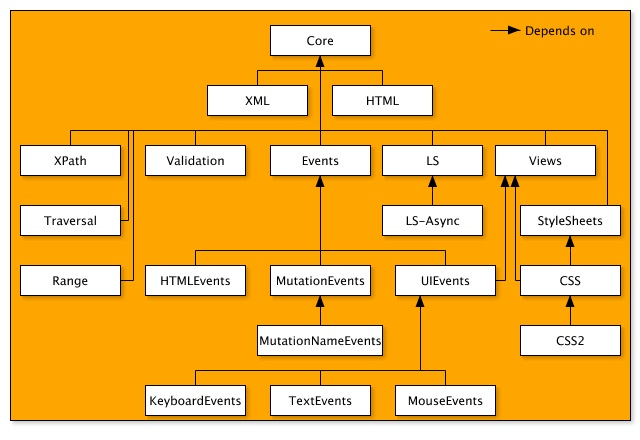
\includegraphics[width=0.65\textwidth]{figures/dom-architecture.jpg}
        \caption{Arquitectura de DOM. Fuente: \cite{w3c}}
        \label{fig:DOM}
    \end{figure}
            
    La interfaz de \textit{DOM} fue definida por el \textbf{OMG IDL} y fue construida para ser usada en una gran variedad de ambientes y aplicaciones. El documento parseado por DOM se transforma en un gran objeto, tal modelo captura la estructura del documento y el comportamiento de éste, además de otros objetos de lo que puede estar compuesto y las relaciones entre ellos. Cada uno de los nodos representa un elemento parseado del documento, el cuál posee una cierta funcionalidad e identidad. La estructura de árbol del DOM construido puede llegar a ser gigantezca, y almacena más de un árbol por cada documento que parsea. 
            
    \subsection{Javascript, VBScript y otros}
    \label{chap2:JS}
    Ambos son lenguajes de scripting orientados a objetos. Javascript fue desarrollado por Netscape mientras que VBScript fue desarrollado por Microsft para Internet Explorer, los dos siguen el estandar del lenguage de scripting \textbf{ECMAScript}. Dado que VBScript no era usado por muchos y no tenía soporte para otros navegadores más que Internet Explorer, Microsoft decidió abandonarlo.

    Muchos piensan que JavaScript es un lenguage interpretado, pero es más que eso. Javascript es un lenguage de \textbf{scripting dinámico} (por tanto no tipificado) que soporta la construcción de objetos basados en \textbf{prototipos}. Esto quiere decir que a diferencia de un lenguage de programación orientado a objetos como Java, un lenguage orientado a prototipos no hace la distinción entre clases y objetos (clase instanciada), son simplemente objetos. Y cómo tal al ser construido con sus propidades iniciales, es posible poder agregar o remover propiedades y métodos de forma dinámica (durante el runtime) tanto a un objeto como a la clase.
            
    Javascript puede funcionar tanto como un lenguage de programación procedural o como uno orientado a objetos. Firefox usa una implementación en C de Javascript llamada \textit{Spider Monkey}, Google Chrome/Chromium tiene un motor de JavaScript llamado \textit{V8} e Internet Explore no usa realmente JavaScript si no que \textit{JScript} (hace lo mismo que las otras implementaciones solo que difiere en el sistema operativo que utiliza) que en este caso se llama \textit{Chakra}.
            
    Si bien es posible comprender que JavaScript posee increíbles posibilidades para la creación de \textit{RIA} (Rich Internet Applications), en \cite{barth2009attacks, Barth2009, Barth2010, Liu2012, Singh2014} se muestran que puede llegar a ser un fracaso si es que no se toman en cuenta ciertas vulnerabilidades inherentes al lenguage. Estas vulnerabilidades que pueden llegar a ser criticas, a menudo permiten a un comunicante comprometer completamente a la otra parte. La misma naturaleza de JavaScript que permite la modificación en runtime de los objetos, puede llegar a ser aprovechada de esta situación; en la cita toma por ejemplo la comunicación entre los elementos de un \textit{Mashup}.


    \subsection{Geolocalización}
    Cada Browser posee una API que permite obtener la data de la localización del host donde el browser está alojado. Ésta es obtenida ya sea del GPS, si es un dispositivo móvil, como de la triangulación de la señal del celular, localización de IP del movil o \textit{access point}.

    \subsection{WebWorkers}
    \label{chap2:WWs}
    Ésta tecnología permite la creación de \textit{threads} en el browser para separar las tareas de éste, dejando algunas en el \textit{background} para incrementar el rendimiento total de la carga de las páginas web. La API permite que el autor de una aplicación web, ejecute \textit{trabajadores} que corren scripts en paralelo, la coordinación entre estos se logra a través del paso de mensajes. Existen 2 tipos: una que es compartida por todo aquello de un mismo \textbf{Origen} y otra que se comunica hacia atrás a la función que la creó. Esta API entrega al desarrollador más flexibilidad, pero que sin duda los atacantes también aprovechan bastante.


\section{Desafíos del Navegador}
    \label{chap2:Desafios}
    \begin{itemize}
        \item Navegación a todo tipo de contenidos/compatibilidad: sin importar el esquema de la página web, el navegador debe ser capaz de presentar todo tipo de contenido al usuario. \cite{barth2008security} asegura que los usuarios demandan compatibilidad, por que el browser es sólo útil mientras pueda mostrar las páginas.
        \item Navegación personalizada: el browser debe ser capaz de entregar la información a la Web Aplicación/sistema, para que identifique al usuario por detrás, de manera que la navegación sea personalizada.
        \item Navegación sin inconvenientes: el navegador debe ser capaz de aislar los errores que se presenten en algunas páginas, de tal manera que no molesten a las otras páginas web que se ven al mismo tiempo \cite{IE8-LCIE, preprint-grosskurth-browser-archevol, barth2008security}
        \item Seguridad: Los datos de los usuarios y el host donde se mantiene el Browser no deben ser expuestos a terceras partes \cite{Reis2009, barth2009securing, Barth2010, Liu2012, barth2009attacks, Saini2014}.
    \end{itemize}


%%%%%%%%%%%%%%%%%%%%%%%%%%%%%%%%%%%%


\section{Arquitectura de Referencia o Reference Architecture (RA)}
\label{chap2:ArqRef}
%usar \cite{Avgeriou2003}

Una arquitectura de Referencia, de acuerdo a la \textit{Open Security Architecture} o OSA \cite{openSecArch}, es considerado un elemento que describe un \textbf{estado de ser} y debe representar aceptadas buenas practicas. En \cite{Avgeriou2003, Galster2011a} se explica que una RA es una arquitectura de software genérica y estandarizada, para un dominio particular e independiente de la plataforma o detalles de implementación. En ésta especifica la decomposición del sistema en subsistemas, las interacciones entre éstas partes y la distribución de funcionalidad entre ellas \cite{Bass2012}. 

Actualmente no hay un consenso de como definir una AR, lo que debería contener y cómo debería de construirse, \cite{Avgeriou2003, Galster2011a} describe un ejemplo e indica como debería de ser ésta con los siguientes elementos:
\begin{itemize}
    \item Describir los Stakeholders que interactuan con el sistema y que poseen \textit{concerns} de éste.
    \item Generar \textit{views} usando UML y teniendo en cuenta un proceso \textit{Rational Unified Process}: crear casos de uso, modelos de análisis y diseño, modelo de despliegue e implementación.
    \item Patrones de Arquitectura.
    \item Atributos de calidad deseables que el sistema debe garantizar. Es importante solo destacar aquellos realmente necesarios, dado que un sistema sobrecargado con ellos tampoco es conveniente.
\end{itemize}

Las ventajas y usos que se obtienen al construir una RA son:
\begin{itemize}
    \item Comprender la estructura subyacente de un Web Browser y las interacciones que tendrá con otros sistemas.
    \item Proveer una base tecnológica modular y flexible. Al tener los subsistemas compartimentalizados es posible quitar y sacar piezas, que poseen interfaces similares, y de esa manera reusar lo otro sin tener que construir un sistema nuevo.
    \item Entrega una base para el desarrollo de otros Navegadores Web, sin explicar detalles de implementación.
\end{itemize}

En este trabajo el enfoque estará en el primer punto, donde se quiere entender las interacciones entre un desarrollo de Software y la utilización de las funcionalidades del Navegador. Dado que parte de la investigación es obtener Patrones de Mal Uso o Uso Indebido del Navegador Web, es primordial concebir una Arquitectura de Referencia que permita encontrar donde es posible aplicar Patrones de Seguridad para poder mitigar los malos usos del Browser \cite{Submitted2014}. 

Una RA es una herramienta que permite facilitar el entendimiento de sistemas complejos y su apropiada construcción a sistemas reales. Si bien una RA es usada principalmente para capturar los \textit{concerns} de los \textit{Stakeholders} al comienzo de un Desarrollo de Software, también puede ser usada para educar al realizar la unión de ideas y terminologías usadas por diversos sistemas que se asemejen. Una Arquitectura de Referencia debe ser en lo posible descrita de la forma más abstracta posible, pues su función guiar la construcción de arquitecturas concretas, sin tener en cuenta detalles de las tecnologías usadas. 

\subsection{Validación de la Arquitectura}
    \cite{Galster2011a} menciona que existe una falta de procedimientos para diseñar sistemáticamente una Arquitectura de Referencia, que sea al mismo tiempo fundamentada empíricamente. El mismo trabajo explica que mientras un Arquitecto de Sistema y un Experto de Dominio trabajen juntos, es posible diseñar AR ya sea desde \textit{cero} o basado en artefactos arquitecturales ya existentes. Para una AR no construída desde el comienzo, la evaluación es menos crítica dado que la AR utiliza conceptos arquitecturales ya comprobados por expertos. Por lo tanto, la validación de ésta puede derivarse desde arquitecturas ya construídas, en este caso a partir de los browser que se encuentran en el mercado.

    Para describir la Arquitectura de Referencia nos hemos basado en los trabajos \cite{Hashizume2014Reference, Submitted2014}, usando patrones para la contrucción de la AR. Así como indica \cite{Bass2012}, es posible usar patrones arquitecturales para diseñar una Arquitectura de Referencia, con tal de obtener atributos de calidad deseados.



\section{Desarrollo de Software Seguro y Diseño de Software Seguro}
\label{chap2:SSD}

La filosofía detrás de \textit{Secure Software Developmet} es que detrás de cada etapa de desarrollo del software, se tengan en cuenta los prinicipios de Seguridad: Confidencialidad, Integridad, Disponibilidad y Auditoría. Para cumplir este cometido es que se deben llegar a políticas y reglas que aseguren la Seguridad como una propiedad sistémica.

Varias comunidades tienen diferentes enfoques y técnicas de cómo asegurar la Seguridad en los sistemas, muchas pueden incluso tener similitudes y hasta trabajar juntas. En este trabajo, el enfoque tomado es aquél que busca entregar la propiedad de seguridad a través del entendimiento de un sistema a un alto nivel, identificando las amenazas durante la elicitación de requerimientos, de manera que se pueda extraer las posibles amenazas que podrían existir y utilizando elementos de diseño para hacer cumplir los principios de seguridad necesarios por el sistema; este enfoque es el que se dedica la comunidad de \textit{Secure Software Design}. 

Fernandez \cite{Fernandez2011a,fernandez2013security} sostiene que para construir un sistema seguro es necesario realizarlo de manera sistemática de tal manera que la seguridad sea parte del integral de cada una de las etapas del Desarrollo de Software - de inicio a fin. El enfoque que propone es ingenieril y por tanto es aplicable incluso para sistemas \textit{legacy}, donde es posible hacer ingeniería inversa para comprobar si existen o no los requerimiento de seguridad implementados, de manera que permite generar un estudio con la intención de comparar y mejorar nuevos sistemas. En su libro \cite{fernandez2013security} presenta una completa metodología para construir sistemas seguros a partir del Diseño Orientado a Objetos, UML y patrones, a los cuales nombra como \textbf{Security Patterns}.

Como parte de la metodología propuesta, se plantea que para diseñar primero se deben entender las posibles amenazas a las que está expuesto el sistema. La identificación de Amenazas \cite{braz2008eliciting,fernandez2006defining} es la primera tarea que presenta la metodología, que considera las actividades en cada caso de uso del sistema.


\section{Patrones}
\label{chap2:Patt}
Los Patrones encapsulan soluciones recurrentes a problemas y definen una forma de expresar los requerimientos y soluciones de una forma concisa, al mismo tiempo que proveen de un vocabulario común entre los diseñadores \cite{buschman1996system}. Un patrón encarna el conocimiento y experiencia de desarrolladores de software que puede ser reusado posteriormente en nuevas aplicaciones \cite{fernandez2004methodology, Fernandez2006, Fernandez2011, fernandez2013security}. Los Patrones expresan las relaciones entre un contexto, un problema y una solución. Para un contexto dado, el patrón puede ser adaptado para encajar en diversas situaciones. La construcción de Patrones de Seguridad parte de la premisa anterior, éste permite construir sistemas seguros a través del uso de Patrones adaptados a las necesidades del sistema y preocupaciones de los \textit{Stakeholders}. Por otra parte, una Arquitectura puede ser descrita a través de Patrones, permitiendo que haya un mejor entendimiento al momento de proveer con guías de diseño y análisis a desarrolladores.

Los patrones describen diseños recurrentes en un mediano nivel de abstraction y es poco probable que existan solos, es decir, existen en conjunto a otros patrones. Un patrón puede proveer una solución usando diagramas en UML, de manera que describen de forma precisa al sistema.

La Arquitectura de Referencia a confeccionar será realizada por medio de patrones y éstos serán descritos con el template creado por \cite{buschman1996system}, llamado POSA, que contiene las siguientes secciones para describir un patrón: \textit{Intent}, Contexto, Problema, Solución, Implementación, Usos comúnes, Consecuencias y Patrones relacionados.




%\section{Patrones de Seguridad}
%\label{chap2:SecPatt}
%Los Patrones de Seguridad son aquellos que encarnan buenos principios de diseño que tienen en cuenta ciertos principios de seguridad, y que al ser aplicados en una metodología para el desarrollo de sistemas, es posible asegurar que el sistema aplique esos principios y en consecuencia generar un sistema seguro \cite{fernandez2004methodology, fernandez2013security}. Estos patrones describen las maneras de detener o mitigar una posible amenaza de seguridad, especificando una solución a través de mecanismos de seguridad, para el contexto dado. Las soluciones propuestas deben resolver las fuerzas o \textit{forces} indicadas por el patrón. Un uso importante de estos patrones es la ayuda que aportan a desarrolladores que no son expertos en seguridad; éstos permiten ayudarlos a implementar mecanismos que implementen los principios de seguridad necesarios.

\section{Patrones de Mal Uso}
Para diseñar sistemas seguros, se es necesario identificar las posibles amenazas que un sistema puede sufrir. Papers como \cite{fernandez2006defining, fernandez2007attack, braz2008eliciting, fernandez2013security} describen el desarrollo de una metodología completa para encontrar amenazas, a través del análisis de actividaddes de los casos de uso del sistema buscando como podría un atacante interno o externo socavar las bases de esas actividades. Es importante no confundir \textit{Attack Patterns} con \textit{Misuse Pattern}, pués claramente en \cite{ModMisusePatt, fernandez2013security} dejan explícito que un \textit{Attack Patttern} es una acción que lleva a un mal uso o \textit{misuse}, o acciones \textbf{específicas} que toman ventaja de las vulnerabilidades de un sistema, como por ejemplo un \textit{buffer overflow}. A partir de los trabajos \cite{fernandez2007attack, yoshioka2006development, yoshioka2007integration}  se hace la unión de los conceptos de \textit{Attack Patttern} para dar forma a la definición de \textit{Misuse Pattern} \cite{ModMisusePatt, pelaez2009misuse, fernandez2010worm, hashizume2011misuse, munoz2011misuse, fernandez2012misuse, alkazimi2014, encinamisuse}:
\begin{center}
    Un patrón de mal uso o \textit{Misuse Pattern} describe, desde el punto de vista del atacante, cómo un tipo de ataque es realizado (qué unidades usa y cómo), analiza las maneras de detener el ataque através de la enumeración de posibles Patrones de Seguridad que pueden ser aplicados, y describe cómo rastrear un ataque una vez que ha ocurrido por medio de una recolección y observación apropiada de datos forenses.
\end{center}

Sin embargo, cuando un sistema ya está diseño y construido, como es el caso del Web Browser, lo que va a importar es saber \textbf{cómo} los componentes del sistema, pueden ser usados por el atacante para alcanzar sus objetivos. Un \textit{Misuse Pattern} o \textbf{Patrón de Mal Uso} describe, desde el punto de vista del atacante, cómo un tipo de ataque es realizado, indicando \textbf{qué} componentes usa y \textbf{cómo}. Además analiza las formas de detener el ataque a través de un listado de posibles \textit{Security Patterns} o \textbf{Patrones de Seguridad} que pueden ser aplicados para esa situación, y describe cómo poder seguir el rastro de un ataque una vez que ha sido realizado con éxito en el sistema, a través de data forense. Además describe un contexto en dónde puede ocurrir el ataque.

Un catálogo de \textit{Misuse Patterns} podría ser de gran valor en el Desarrollo de Sistemas que interactúan con el Navegador, pués provee a desarrolladores un medio para evaluar los diseños de sus sistemas, al analizar las posibles amenazas del Browser que pusieran afectar al software que está siendo construído.

\newpage
\chapter{Marco Teórico - (In) Seguridad en el Browser}
\label{chap3:MT}

En esta sección se presentan los posibles ataques que un \textit{Browser} puede sufrir y que directamente podrían afectar al sistema con el que se comunica. Principalmente ahondaremos en los ataques en el \textit{Browser} relacionados a las técnicas de Ingeniería Social \cite{socEngineeering}. El escenario actual de los ataques en el \textit{browser} ha cambiado bastante, si es comparado a aquellos de la decada de los noventa. Cada día los Browsers son más robustos y difíciles de explotar, y por lo mismo los ataques de tipo \textit{drive-by downloads} o los basados en ejecución de código para vulnerar el sistema, cada vez son menores. Una nueva forma de ataque ha emergido y es bastante fácil de lograrlo, pues se basa en el engaño del usuario a realizar lo que el atacante desea. Una vez el usuario es engañado, el atacante puede lograr un control total tanto del \textit{Browser} o del Host, sin haber tenido que vulnerar el sistema \cite{Rajab2013} que aloja al \textit{Browser}. Desarrollos de sistemas críticos que interactuan a diario con diferentes usuarios en la red, deberían de ser los más preocupados de estos ataques pues atentan contra la confidencialidad, integridad y disponibilidad de los datos, tanto del usuario (personales) como los de los \textit{Stakeholders} involucrados.

\section{Social Engineering o Ingeniería Social}
\cite{socEngineeering} define este tipo de acción como: El acto de manipular una persona para realizar acciones que no son parte de los mejores intereses del \textit{blanco o víctima} (la misma persona/organización/etc u otra entidad). Un ataque de éste tipo puede darse de diversas maneras, no dejando la posibilidad de un encuentro físico o digital con el que realiza el engaño. Un ataque basado en ingeniería social, es uno que se aprovecha del comportamiento humano y la confianza de la víctima. En el contexto del Web Browser, el usuario engañado es la primera y última línea de defensa contra este tipo de ataques, pues un abuso en la confianza del usuario podría abrir las puertas al Host del \textit{Browser}, logrando un daño tanto del usuario como con los sistemas externos con los que interactúa.

\section{Ataques y Amenazas}
Esta sección incluye algunos ataques posibles de realizar en un \textit{Browser} y que podrían afectar tanto directa como indirectamente a un sistema externo. Acá no incluiremos ataques en donde el Host ya ha sido vulnerado con anticipación, o aquellos que puedan correr software con los privilegios de un usuario del sistema Host, es decir, aquellos donde el Host ya ha sido controlado directamente por medio de alguna vulnerabilidad del sistema. En el caso anterior, los Browsers ya nada pueden hacer para detener un ataque de esa magnitud.

En el Top Ten \cite{owaspTopTen} de la OWASP (Open Web Application Security Project) - los diez riesgos de seguridad más importantes en Aplicaciones Web - se puede distinguir en el año 2013 los riesgos directamente relacionados a amenazas de seguridad en el \textit{Browser}. Algunos como: Injección (A1), Manejo de sesiones y autenticación roto (A2), XSS (A3), CSRF (A8) y uso de componentes con vulnerabilidades conocidas (A9), son los riesgos que las organizaciones podrían sufrir en sus sistemas cuando se realizan ciertos ataques en el \textit{Browser}.

En trabajos \cite{barth2008security, FirefoxThreatModel} se puede apreciar los Threat Model para los Navegadores Chromium y Firefox respectivamente. Es posible observar que existen ataques que pueden generar secuelas en otros sistemas, si es que el Navegador es afectado en primera instancia. Algunas amenazas existentes relacionadas con los riesgos mencionados en el párrafo anterior son:

\begin{enumerate}
	\item Compromiso de los componentes del Navegador (plugins incluídos) que poseen privilegios de usuario.
	\item Compromiso del Host/Sistema.
	\item Robo de datos en una red.
	\item Compromiso de páginas web (y su data) de origenes distintos.
	\item Fijación de sesión o robo de ésta
	\item Compromiso de los canales de comunicación del \textit{Browser}.
\end{enumerate}

Una lista (parcial) de ataques asociados a las amenazas anteriores son:

\subsection{Phishing}
Este ataque consta principalmente del engaño al usuario, confundiendolo a que visite una página deshonesta en vez de la que tenía pensado; es uno de los tantos ataques que usan la ingeniería social para dañar a un usuario. En el estudio realizado por NSS Labs \cite{browSecPhish} afirma que muchos de los ataques que actualmente están ocurriendo se han limitado al uso de técnicas de ingeniería social. Si bien los ataques basados en drive-by downloads y clickjacking siguen siendo de alto impacto, los atacantes parecen preferir los otros por la simplicidad de éste, pues no es necesario conocer realmente vulnerabilidades del \textit{Browser} para llevarlos a cabo. 
	\subsubsection{Instalación de Malware o Extensiones malignas}
	Un ataque de este tipo puede ser originado desde la ejecución de un ataque Phishing a una persona; en especial cuando se hace creer que lo que se va a instalar, es completamente inofensivo.

\subsection{XSS - Cross-Site Scripting DOM}


\subsection{Man in the \textit{Browser} (MITB)}



\section{Mecanismos de Defensa que se espera que el Host del \textit{Browser} tenga previamente}
	Antes de revisar los mecanismo que un Navegador nos ofrece, es importante 


\section{Mecanismos de Defensa del \textit{Browser}, para los ataques revisados}

\subsection{Sandboxing de procesos/componentes}
    \label{chap3:Sandboxing}
    La idea es encapsular el área de mayor probabilidad de ataque en un espacio aislado, minimizando la superficie de ataque de un software. Sandboxing no es una técnica tan nueva, han existido sistemas que ya lo han incorporado. Ésta protección puede ser aplicada dependiendo del diseño del software, algunos ocupan Sandbox a nivel del sistema operativo como otros que ocupan al nivel del \textit{engine} de Javascript. En el caso especial del \textit{Browser}, esta técnica es construida en el nivel más alto posible para un programa de usuario, lo que permite la separación de privilegios entregados por el sistema operativo al \textit{browser} y los subprocesos que corren dentro de éste. El atacante que se enfrente a un \textit{browser} que tenga este mecanismo de defensa, tendrá que realizar primero un \textit{bypass} encontrando una vulnerabilidad en el sandboxing del \textit{browser}. Existen diferentes técnicas para Sandboxing, todo depende del diseño del \textit{Browser}.

    %Hablar del sandbox de IE y Chrome, Firefox no tiene

 \subsection{Aislación del contenido web de los componentes del \textit{Browser}}

 \subsection{Blacklist y Whitelist de sitios web}

 \subsection{Detección de Malware por medio de sistemas de Reputación}


\newpage
\chapter{Browsers y Estado del Arte}
\label{chap4:EA}


\section{Arquitectura de Referencia del Browser y Patrones}
\label{chap3:ArqRefBrowandPatt}

%Decir: "este trabajo es basado en la metodología de Fernandez \cite{Hashizume2014Reference} usando patrones en la construcción de la arquitectura de referencia"

\subsection{Método}
El primer paso para realizar el estado del arte con respecto a este punto fue realizar una búsqueda ordenada y a través de string de búsqueda dentro de web engines y librerías digitales conocidas. Se utilizaron las siguientes plataformas para buscar documentación al respecto:
\begin{itemize}
    \item Google, usando \textit{google dorks} para filtrar resultados
    \item Scopus y Google Scholar, usando string de búsqueda y operadores booleanos para filtrar resultados.
\end{itemize}

Para aquellos buscadores donde era posible usar operadores booleanos también se trató de filtrar el contenido para que pudiera mostrar resultados relacionados a: \textit{Browser} y \textit{Reference Architecture}. Sin embargo los resultados fueron bastante pobres. Desafortunadamente hasta la fecha no existen muchos trabajos relacionados a la construcción de una Arquitectura de Referencia para el Browser. Dado que la búsqueda no entregó muchos resultados, se procedió a hacer un \textit{forward snowballing} con el único paper que creemos entrega información similar a lo que se buscaba. Sin embargo, tampoco encontramos tanta información.

\subsection{Lo encontrado}
%larrondo
En Larrondo-Petrie et. al \cite{535061} se realiza un análisis del web browser, con el fin de obtener un Modelo de Dominio, un Modelo de Objetos y un \textit{Feature Tree} que describiera la estructura y funcionalidad entregada comúnmente por los Web Browser. El dominio, según explica el trabajo, es un set distintivo de objetos que se comportan de acuerdo a reglas y política que caracterizan el Dominio. El Análisis de Dominio es realizado para identificar dominios y cómo estos interactuan con otros. La metodología usada para obtener los Dominios es el \textit{Object Oriented Analyis}. Además de identificar, se clasifican estos dominios de acuerdo a su rol en el sistema terminado como: Dominio de Aplicación, Dominio de Servicio, Dominio de Arquitectura y Dominio de Implemntación. El Modelo de Objetos sirve para entregar más detalles, un resumen general de las Entidades del Web Browser y sus relaciones. El Feature Tree pretende entregar detalles sobre los aspectos funcionales de la aplicación. El Modelo planteado, śegún el artículo, debería ser útil para los Desarrolladores de Software que construyen \textbf{Aplicaciones Web basadas en el uso del Browser}.  Este estudio se encuentra bastante lejos de lo que se quiere hacer en este trabajo, pero sirve para obtener un transfondo de lo que sucede en el Web Browser, aún cuando la información esté muy desactualizada.

% preprint-grosskurth-browser-archevol y 2005-grosskurth-browser-refarch

En el trabajo de Grosskurth et al. \cite{2005-grosskurth-browser-refarch, preprint-grosskurth-browser-archevol} se utiliza una herramienta de ingeniería inversa, para obtener una arquitectura de referencia de muy alto nivel en base a dos navegadores open-source: Mozilla y Konqueror. Lo obtenido captura los subsistemas fundamentales comunes a los sistemas del mismo dominio, así como las relaciones entre estos subsistemas. En esta arquitectura se identifican los siguientes subcomponentes: Interfaz Usuaria, Persistencia de Datos, Browser Engine, Rendering Engine, Networking, Interprete de Javascript, XML Parser y Display Backend. Se menciona que estos componentes están estrechamente integrados (high coupling) con el Rendering Engine, lo cuál tiene sentido en la arquitectura monoproceso que poseen Mozilla y Konqueror; es una decisión de diseño muy común en los Browser de la época. Al identificar estos componentes, se comenta que ésto podría servir tanto en el diseño y durante la mantención de un sistema, pues mejora el entendimiento de un sistema al ayudar a analizar los trade-off entre diferentes opciones de diseño; o también puede servir como un template para obtener nuevos diseños. Una vez obtenida la arquitectura conceptual, se inició una evaluación de ésta al comparar las arquitecturas concretas de cada browser open-source, extraídas desde el código fuente, para ver que tanto el modelo conceptual era cercano a la realidad; la constante comparación permitió ademas refinar Arquitectura de Referencia. Los browsers usados para validar fueron: Epiphany, Safari, Lynx, Mosaic y Firefox. Si bien la arquitectura entregada entrega bastante información a alto nivel, no desarrolla más que esa capa de abstracción, además parece ser que depende también de la implementación usada en la herramienta de ingeniería inversa. 


%Godfrey2000
En el documento \cite{Godfrey2000} realizado en el año 2000, se describe la experiencia realizada al extender el rabajo del proyecto TAXFORM. Usando PBS, una herramienta de Ingeniería Inversa, se extrajo la arquitectura de software del Navegador Mozilla, con el objetivo de entender la estructuración de sus componentes; además de crear vistas arquitecturales de alto nivel del sistema. El modelo arquitectónico obtenido contiene 11 subsistemas de alto nivel, de éstos los que más se destacaron fuer el \textit{HTML Layout}, la implementación de herramientas y el código de la interfaz de usuario. En el año en que se lleva a cabo este estudio (2000), se menciona que la arquitectura ha decaído significativamente en muy poco tiempo, o su arquitectura no fue planificada cuidadosamente desde el comienzo; parte de lo anterior, el autor cree que es secuela de la \textit{Guerra de Navegadores}. Si bien el trabajo ayuda a entender un poco la estructura detrás del navegador, este trabajo es muy antiguo y la versión más actual del navegador ha cambiado bastante. Además lamentablemente, el enfoque de este estudio no es intentar entender lo que hace cada subsistema, si no que es la implementación de la herramienta misma para obtener la arquitectura de software del browser seleccionado.

%Lwin2009 - Agent Based Web Browser
En \cite{Lwin2009} se propone un Browser llamado Anfel SOFT, donde gracias al uso de Inteligencia Artificial, crea agentes que permiten mejorar la experiencia del usuario. El trabajo asegura que el browser será capaz de aprender el comportamiento de navegación del usuario, y guiará al usuario en su navegación para que esta sea lo más efectiva posible. El paper obtiene los subsistemas que se pueden encontrar en un browser de la misma manera que lo realiza \cite{2005-grosskurth-browser-refarch}. Si bien la arquitectura que muestra refleja parte de lo visto en los 3 browsers escogidos en este estudio, no da detalles acerca de cada subsistema identificado. Además la arquitectura de Referencia que entrega es la misma vista en \cite{2005-grosskurth-browser-refarch, preprint-grosskurth-browser-archevol} y a pesar que identifica otros posibles componentes, no agrega nada nuevo.

Podemos ver en los trabajos que algunos construyen una Arquitectura de Referencia basada en técnicas de Ingeniería Inversa. En cada uno de ellos el trabajo ha sido a muy alto nivel y la descripción de los subcomponetes del sistema es mínima. Si bien explican las relaciones entre éstos, no dan un mayor entendimiento en como se comportan en ciertas situaciones. En este trabajo se espera profundizar un poco más en la abstracción obtenida, incluyendo información de tanto los casos de uso del Browser como las actividades que se realizan con otros usuarios. Desafortunadamente para esta memoria no existe mucha literatura sobre el desarrollo de una Arquitectura de Referencia del Browser, y de lo que hay el trabajo más actual es el realizado por \cite{Lwin2009} en el año 2009.


\section{Google Chrome y Google Chromium}
    \label{chap3:GC}
    La misión de Google es organizar la información del mundo y lograr que sea útil y accesible para todo el mundo. Esta gran empresa partió como un búscador y rápidamente llegó a ser dueño de la mayor parte de búsquedas del mercado. Tiene servicios de almacenamiento en la nube, correo electrónico, \textit{e-wallet} y otros más. Google ha sido responsable por la construcción del Navegador Web \textbf{Google Chrome} y \textit{Google Chromium}. En el 2008, Google liberó gran parte del código de Chrome bajo el proyecto de nombre Google Chromium, el cuál es open-source que permitiría a desarrolladores \textit{third-party}, estudiar el código fuente y ayudar en la implementación para las plataformas Linux y OS X. La diferencia entre Chrome y Chromium son: actualizaciones automáticas y Adobe Flash integrado (aunque éste último ya se está cambiando el uso por HTML5). En  \cite{EvolutionofWeb} se menciona que este Navegador ha sido el último que ha salido y se llevado una gran parte del mercado \cite{statBrow}.

    La arquitectura de Chrome o Chromium se basa principalmente en dos módulos: el Browser Kernel y el Rendering Engine, cómo se puede ver en la Figura \ref{fig:archG}.

    \begin{figure}[h!t]
        \centering
        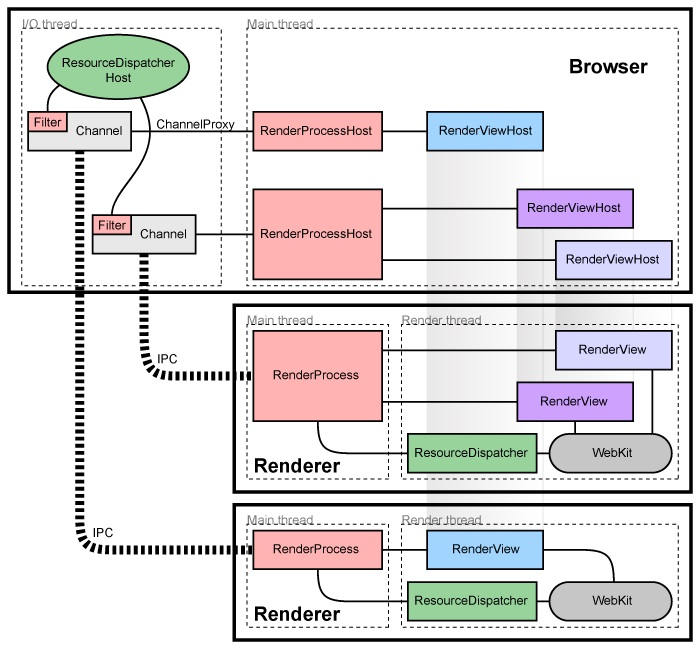
\includegraphics[scale=0.5]{figures/archGC.jpg}
        \caption{Architectura Multi procesos de Google Chrome. Fuente: \cite{multiProcGC}}
        \label{fig:archGC}
    \end{figure}

    Én la documentación de Google Chromium \cite{multiProcGC}, que es base para Google Chrome, afirma que la arquitectura soporta para cada tab un proceso nuevo, de manera de hacer al Browser más robusto y modularizar el sistema para evitar ciertas amenazas de seguridad. El proceso principal es llamado \textit{Browser Process/Kernel/Engine} y se encarga de la \textit{User Interface}, manejo de las tabs y los procesos de los \textit{plug-in}. Cada tab es asociado a un Rendering Engine, éstos tienen restricciones de acceso (\textit{Sandoboxing}) a los demas y al sistema, lo que permite que exista una protección de la memoria y un control de acceso. Google Chrome expone en \cite{reis2009browser} que existen ciertas lecciones que han ido utilizando para mejorar la calidad de su browser. Estas son:

    \begin{itemize}
    	\item Reducción de las vulnerabilidades de seguridad, se basa en la aislación de ciertos componentes y la reducción de privilegios de ciertas tareas en el browser. La aislación lo lograron con la creación del Rendering Engine y el Browser Kernel, que tienen como objetivo proteger la data del sistema de archivos. Si bien esto puede no entregar muchos beneficios a una aplicación web, si lo hace en el usuario del browser.
    	\item Reducir la ventana de vulnerabilidades, la actualización del browser se hace cada cierto tiempo de forma automática para así cubrir las vulnerabilidades que van apareciendo.
    	\item Reducción de la frecuencia de exposición, Google trabaja con StopBadware.org para entregar una mayor seguridad al descubrir nuevos tipos de ataques y vulnerabilidades relacionadas con el browser.
    \end{itemize}

    En \cite{barth2008security} se explica que el objetivo principal de esta arquitectura es poder mitigar ataques muy severos sin tener que sacrificar la compatibilidad con los sitios web ya existentes. Para lograr el objetivo Google ha ganado muchas lecciones de cómo realizar esto \cite{reis2009browser}, pues explican que un gran desafío en la seguridad es proteger a los usuarios de los atacantes que se aprovechan de las vulnerabilidades y debilidades de los clientes web-browsers. En su arquitectura modular se puede ver que se intenta proveer una seguridad que evita afectar la compatibilidad con otros sitios. La arquitectura comentada se basa en dos decisiones de diseño: La arquitectura depende en el Rendering Engine para aquellos componentes de alto riesgo como JavaScript, el parser de HTML y la creación de DOM para hacer cumplir SOP; al estar rodeados por un Sandboxing hace que el Rendering Engine se comporte como una caja negra. 

 \subsection{Browser Kernel/Process y Renderering Engine/Process - Blink}
    El Browser Process provee al usuario con lo necesario para el manejo de sesiones (cookies, tokens, etc), historial, almacenamiento de passwords, manejo de interfaz de usuario, barra de localización, sistema local de blacklist, API para realizar llamadas al sistema tanto para almacenar datos como para realizar request del usuario, agente de descarga, entro otros. El Browser Kernel tiene la tarea de ser un interceptor de las llamadas de los procesos Rendering que están un Sandbox, revisando las políticas y qué acciones están permitidas.

    \begin{figure}[h!t]
        \centering
        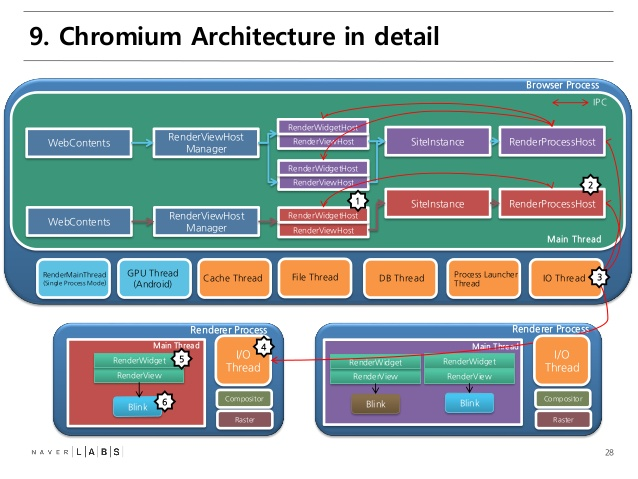
\includegraphics[scale=0.5]{figures/chromium-rendering-pipeline-28-638.jpg}
        \caption{Architectura de Chromium en detalle. Fuente: \cite{ChrRenderPipe}}
        \label{fig:archGC2}
    \end{figure}

    El \textit{Rendering Engine} usado por Google Chrome/Chromium, llamado Blink, es un \textit{forking} del trabajo original llamado Webkit. Su objetivo principal es soportar la architectura de multi-procesos que posee el navegador y al mismo tiempo poder reducir el nivel de complejidad. Cada nueva ventana o tab abre un nuevo proceso, y el Browser instruye a ese proceso a crear un componente que permitirá la visualización del recurso en el navegador. Cada proceso abierto para instanciar un Renderer estará en Sandbox, donde puede pasar que 2 tabs de diferentes dominios estén en el mismo proceso, dado que puede haber una relacíón en la navegación de éstas páginas.


    %     \begin{figure}[h!t]
    %     \begin{center}
    %         \includegraphics[scale=0.5]{figures/in_process_plugins.png}
    %       %\caption{Representación conceptual de una Nube con Eucalyptus. La especificación de las partes y su explicación se ve en \ref{sec:chap2.4.2}. Fuente \cite{EucalyptusOverview}}
    %       \label{fig:archG}
    %     \end{center}
    % \end{figure}

    %\subsection{Extensions}

    %\subsection{Plugins}
    %En el ultimo tiempo, los plugins como Adobe Flash

\section{Internet Explorer}
    \label{chap3:IE}
    Internet Explorer es el navegador grafico predeterminado por Microsoft y que su primera versión 1.0 fue realizada en 1995. IE es una derivación de Spyglass Mosaic desarrolado por la NCSA (National Center for Supercomputing Applications). En primera instancia fue un navegador que podría ser obtebido si era comprado como complemento de \textit{Microsoft Plus!} o mediante la versión \textit{OEM} de Windows 95. Desde la tercera versión de IE, en 1996, que esta se lanzó de forma gratuita.
            
    La arquitectura de este navegador es modular y permite al desarrollador por utilizar los recursos para crear diferentes funcionalidades, ejemplo de esto son: toolbars, Microsoft Active X controls, etc. En la Figura \ref{fig:archIE} \cite{IEArch} se puede ver los principales componentes de la architectura del browser mencionado. IE utiliza \textit{COM} o \textit{Component Object Model} una interfaz binaria standard para componentes de software introducida por Microsoft en 1993 y que permite una comunicación entre procesos/componentes de software provenientes de la familia de software de Microsoft. \textit{COM} es similar a otras tecnologías de interfaz de componentes de software ( Component Software Interface Technologies) cómo CORBA y Java Beans. El uso de \textit{COM} gobierna la forma la interacción de los componentes que se comunicann y permite que haya un reuso y extensibilidad de estos.
            
	\begin{figure}[h!t]
	    \centering
		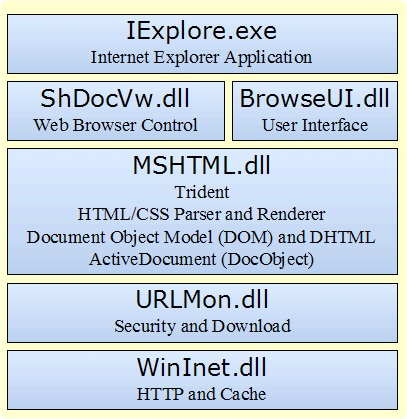
\includegraphics[scale=0.65]{figures/IEArch.jpg}
		\caption{Arquitectura de Internet Explorer. Fuente: \cite{IEArchImg}}
		\label{fig:archIE}
    \end{figure}

    \begin{figure}[h!t]
        \centering
        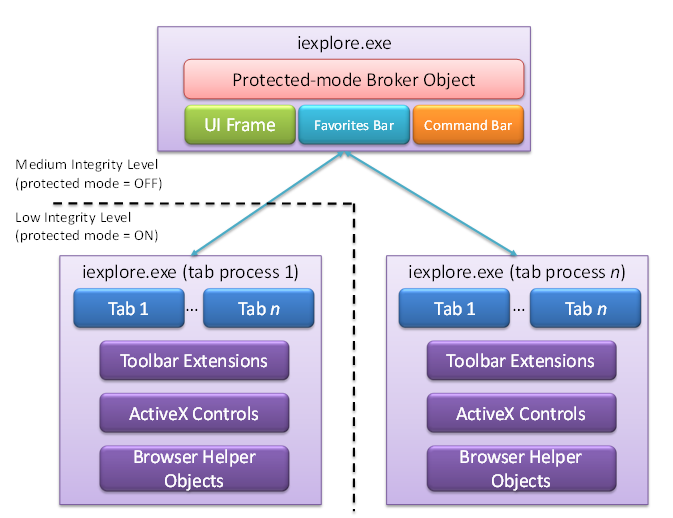
\includegraphics[scale=0.5]{figures/11_IE8andLooselyCoupledIELCIE_2.png}
        \caption{Arquitectura de Internet Explorer más detallada. Fuente: \cite{IE8LCIE}}
        \label{fig:archIE2}
    \end{figure}

    \subsection{Frame Process y Rendering Engine}   
        \label{chap2:Trident}
        O también llamado MSHTML, es un rendering engine privativo, sin embargo es posible usarlo al usar librería de Windows \textbf{mshtml.dll}. Según \cite{Crowley2010} es un objeto OLE (Object Linking and Embedding) Active Document que representa el \textit{layout} de Internet Explorer y permite mostrar graficamente las páginas por medio del \textit{display} del host. Dentro de éste se manejan las Extenciones, el \textit{engine} de Javascript y la librería que contiene la API para tareas de \textit{networking}, además de proveer una capa de seguridad y manejar las descargas de archivos.

    %\subsection{HBO}

    %\subsection{Plugins}


\section{Firefox}
    \label{chap3:Firefox}

    Firefox fue creado a partir del navegador \textit{Netscape} en 1998, actualmente la fundación Mozilla ha sido la que la ha mantenido, generando varias modificaciones desde su nacimiento. Las metas de diseño que Mozilla desee en el navegador son:
    \begin{itemize}
        \item Renderizado rápido de las páginas web.
        \item Fuerte apoyo a los estandares web como la W3C.
        \item Interoperabilidad en las diversas plataformas.
    \end{itemize}

    \subsection{Firefox Mono-proceso y Gecko}
        \begin{figure}[h!t]
    		\centering
        	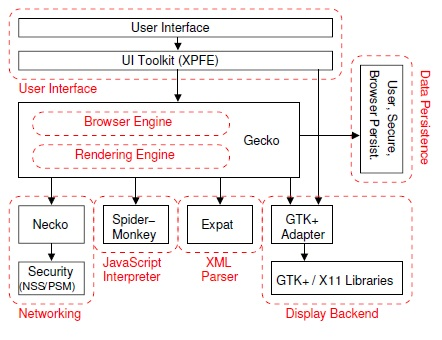
\includegraphics[scale=0.8]{figures/archMoz.jpg}
            \caption{Arquitectura Monoproceso obtenida en Fuente \cite{2005-grosskurth-browser-refarch, preprint-grosskurth-browser-archevol}}
            \label{fig:archM}
        \end{figure}
                
        La arquitectura de este browser puede ser vista en la Figura \ref{fig:archM} donde se pueden observar los siguientes componentes principales:
                \begin{itemize}
                    \item La interfaz de usuario, la cuál puede ser reutilizada para otras aplicaciones por su bajo coupling con el sistema entero. 
                    \item La persistencia de los datos, tanto de bookmarks como de data de bajo nivel como el \textit{cache}.
                    \item EL \textit{Rendering Engine}, permite el renderizado de documentos HTML/XML por un tipo de parser basado en web standardds. Este Engine es capaz de renderizar la interfaz de la aplicación multi-plataforma.
                    \item XPCOM
                \end{itemize}
        La arquitectura de Mozilla se distingue de las demás en que la visualización especificada por la plataforma y la librería de \textit{widgets} son usados directamente en el navegador, lo que minimiza el costo necesario para soportar diferentes plataformas. Si bien esta figura muestra lo más importante, algunos detalles relevantes son olvidados, como las extensiones y el componente XPCOM (cross, platform component object model) que es similiar al componente COM de Microsoft,

        Gecko es un motor de renderizado \textit{Open Source} que utiliza Firefox, escrito en C++, creado en un comienzo por Netscape, predecesor de Mozilla Foundation/Corporation. La función de este componente en Firefox (y otros browsers que lo integran) es leer el \textit{web content} de tipo HTML, CSS, XUL (para renderizar \textit{User Interface}) y Javascript, y mostrarlo al usuario en un formato gráfico. Tiene un gran rendiemiento al transformar a formato gráfico una página con lenguaje de marcado ya que soporta multithreading en el parser de HTML. Gecko fue diseñado para soportar \textit{Open Internet Standards} y por ende sigue al pie de la letra todas las especificaciones de HTML 4, CCS 1 y 2, DOM, XML y Javascript. Los componentes de Gecko incluyen:
            \begin{itemize}
                \item Parser de Documentos (HTML y XML).
                \item \textit{Layout Engine} con un modelo de contenido; ésta es la información que el display del host mostrará al usuario.
                \item Sistema de estilos.
                \item Motor de Javascript. En el caso de Gecko éste se llama \textbf{SpiderMonkey} que está escrito en C/C++.
                \item Librería de imágenes.
                \item Librería de \textit{Networking} o Necko.
                \item Renderizado gráfico específico a la plataforma y widget de acuerdo al sistema operativo.
                \item Librerías de Seguridad, NSS
                \item Mozilla Plug-in API (NPAPI).
                \item Lbrería de preferencias de usuario, entre otros más.

            \end{itemize}
        En la figura \ref{fig:Gecko} se explica como el Rendering Engine es capaz de crear una página a través de un HTML y su correspondientes CSS. Éste parte como 2 pipelines que leen tanto HTML como CSS, y cuando llegan al Frame Constructor se vuelven una. Ya en esa fase, se espera que solo una hebra se encargue del contenido visual que se mostrará, pues si se tuviera más habría problemas con las prioridades de los elementos a mostrar en el DOM y el Layout final.

        Finalmente, en el día de hoy los Plugins ya son considerados tecnología \textit{legacy}, en especial el uso de Adoble Flash, que estaba bien arraigado, ahora se ha empezado a utilizar HTML5 como una alternativa que se ajusta a los estándares de la W3C.

        \begin{figure}[h!t]
            \centering
            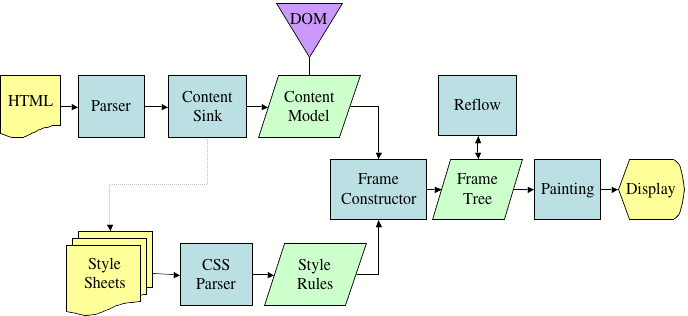
\includegraphics[width=0.8\textwidth]{figures/Gecko_Overview_9.png}
            \caption{Gecko Rendering Engine. Fuente: \cite{gecko}}
            \label{fig:Gecko}
        \end{figure}

        \subsubsection{Estabilidad y Recuperación a fallos}
        Este tipo de Firefox utiliza un proceso que se encarga de realizar tanto el Renderizado como la comunicación con las páginas web, y tiene la desventaja de que si sufre un fallo pequeño, todas las Tabs asociadas al proceso pueden ser corrompidas por el fallo. Así como también, el cierre inesperado puede causar una perdida total de los datos. Aunque Firefox sea uno de los Browser con mejor compatibilidad y sigue bastante bien los Web Standards de la W3C, le ha sido bastante dificil moverse a una arquitectura Modular como Google Chrome Y Explorer \cite{ElectrolysisTalk}
        
    \subsection{Firefox Multi-proceso (Electrolysis, e10s)} 
    Éste proyecto comenzó el 2009 y que por motivos desconocidos \cite{ElectrolysisTalk} se tuvo que poner en espera el proyecto. El 2012 la Arquitectura del Sistema Operativo Firefox empezó a usar la idea de multiprocesos que se había estado trabajando, por lo que el 2013 se recontinuó el proyecto, sin embargo aún no hay una versión estable y solo se puede ocupar como testing en la versión Nightly Build \cite{NightlyBuilds}. La nueva Arquitectura se basa en usar la aislación que provee el sistema operativo a los procesos, de la misma manera que lo hace Google Chrome, pero por supuesto el diseño no es el mismo.

    \subsubsection{Chrome Process y Content Process}
    Respecto a este componente de la nueva arquitectura que Electrolysis, no mucha información de que es lo que hace está en linea. Parte de los componentes son el sistema de comunicación que existe entre los procesos o Message Manager, que se encarga de enviar mensajes de control desde el Chrome Process a los procesos hijos o recibir los mensajes desde sus procesos hijos para realizar las acciones necesarias para mostrar el contenido.
        \begin{figure}[h!t]
            \centering
            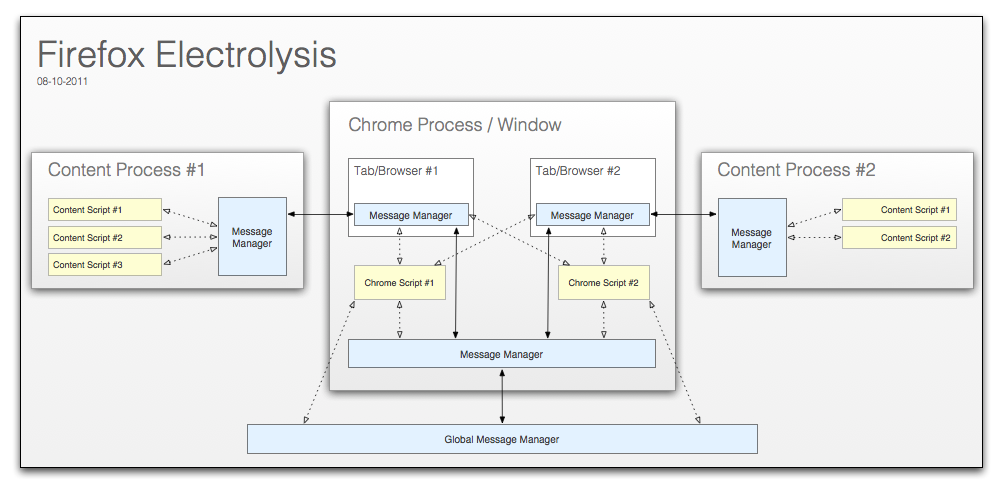
\includegraphics[width=0.8\textwidth]{figures/electrolysis.png}
            \caption{Firefox Electrolysis, communication 1. Fuente: \cite{Firefox101}}
            \label{fig:ChromePComm1}
        \end{figure}

    Así como Google e Internet Explorer, se tiene al Chrome Process como intermediario para cualquier tipo de acción dentro del Browser lo que permite controlar las peticiones del usuario o scripts que se ejecuten en el Content Process (hijo).

        \begin{figure}[h!t]
            \centering
            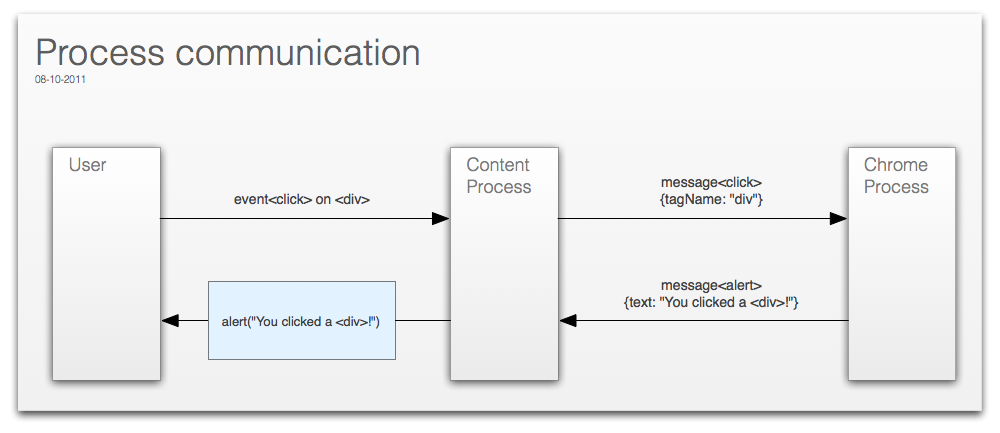
\includegraphics[width=0.8\textwidth]{figures/e10s-processes.png}
            \caption{Firefox Electrolysis, communication 2. Fuente: \cite{Firefox101}}
            \label{fig:ChromePComm2}
        \end{figure}

    Esta propuesta, si bien ha capturado buenas prácticas aún no ha podido realizar una implementación del Sandbox y está lejos aún.


% \subsection{Rendering Engines}
% \label{chap2:RenderingE}
% Responsable de converitir la página web, en HTML o XML, a un formato visible cómodo para el usuario en la pantalla del host. La combinación de HTML, CSS y media (imagenes, videos, etc.) permiten entregar una experiencia gráfica al usuario con la que interactuará. Existen browser que no usan gráficos y solo se basan en mostrar texto, ejemplos de estos navegadores son: W3M y Lynx. Los \textit{Rendering Engines} más usados son: Webkit (Safari), Blink (Google Chrome/Chromium), Trident (Internet Explorer) y Gecko (Firefox).

%     \subsubsection{Trident}
%     
%     








\newpage
\chapter{Definición de una Arquitectura de Referencia para el Web Browser}
\label{chap5:ArqRefWB}


Para poder entender algún Browser se buscó en específico trabajos, papers, documentación gris a través de buscadores web como: IEEE Xplore, ACM digital Libray, Scopus y otros más, con tal de encontrar documentos formales sobre sus arquitecturas. Lo que más se encontró fueron blogs de desarrollo y White papers sobre Google Chrome, sin embargo llama la atención la escases en literatura sobre el tema. 


En vista a la poca, casi nula, documentación formal sobre el Navegador Web, la necesidad de hacer una Arquitectura de Referencia (AR) para entender cómo la arquitectura de este sistema puede relacionarse con el futuro desarrollo de otros sistemas, puede llegar a ser de gran utilidad para explicar los conceptos de seguridad detrás del Navegador. Se sabe que el Browser es un pieza de Software que ha sufrido varios cambios desde la década de los 90, por lo tanto entre los desarrolladores de esta herramienta ya existen convenciones de qué elementos funcionan mejor. Por consiguiente, no es de extrañar que diferentes browsers estén construidos de formas muy similares, y puedan ser conceptualizados en una AR que manifieste los componentes, mecanismos de comunicación y funciones de esta pieza de Software. 


La AR a construir en este trabajo, fue realizada principalmente a través de la abstracción de las propuestas actuales de los Web Browsers más usados: Google Chrome, Internet Explorer y Firefox (propuesta Electrolysis). Primero se identificarán y analizarán los stakeholders, se identificarán los casos de uso relacionados a cada uno de estos stakeholders y se dará una descripción breve. Se han identificado 3 patrones: Browser Infrastructure, Web Content Renderer y Browser Kernel. El primero corresponde a la infraestructura completa del Browser, mientras los otros dos son subsistemas internos que en conjunto forman el Navegador. Para este trabajo solamente se desarrollará el patrón que representa el sistema completo, es decir, el patrón Browser Infrastructure; en éste están los componentes principales, la comunicación con el host y la interacción entre éstos. El patrón Browser Insfrastructure será descrito utilizando un template POSA \cite{buschman1996system} y notación UML para precisar cómo en una AR se relacionan los componentes. 

\section{Casos de Uso del Browser}
	\subsection{Stakeholders (actores) y Concerns de estos}
	Se es necesario encontrar los actores (definido por sus roles) que participan en el uso y operación del Navegador, éstos son:
		\subsubsection{Browser User (BU)}
		En principio, representa a un usuario del Host que utiliza el Navegador. De este stakeholder depende que se realice el inicio de una petición para buscar una página web, recurso o servicio (Sin éste la utilidad del Web Browser es nula). Puede tratarse de una entidad no humana, como un plugin, extensión o instancia de una página web, pueden requerir hacer peticiones por medio de las interfaces del navegador, con la intención de cumplir con el deseo del usuario del host de mostrar el contenido en el Browser.
		\subsubsection{Host (H)}
		Para este caso nos referiremos solamente a la máquina cliente dónde se aloja el Web Browser. Ésta crea los procesos necesarios para iniciar el Navegador, además de entregar un ambiente al Browser para que éste pueda funcionar adecuadamente.  Esta identidad se encarga de aplicar políticas de seguridad sobre el Browser cuando se necesiten realizar operaciones o el navegador desee crear nuevos procesos.
		\subsubsection{Provider (P)}
		Es toda la infraestructura relacionada con el Servicio Web que pudiera entregar una máquina remota a un Navegador. Este puede ser un: Web Server, Web Aplicación, Servicio de actualización del Browser, etc. Su interacción con el Browser se limita a entregar contenido a éste.
		\subsection{Casos de Uso}
Los casos de usos y actores están listados a continuación. Notar que se presentarán aquellos casos de uso relacionados exclusivamente con el Browser.

\subsubsection{Casos de Uso para Browser User (BU)}
		El BU representa todas las interacciones posibles del usuario con el Browser y sin él no habría razón para la existencia del navegador; un servidor tampoco existiría dado el mismo principio. Al encontrar los casos de uso de este stakeholder veremos las preocupaciones de éste, lo que nos permitirá entender las necesidades de seguridad para proteger al navegador. Los casos de uso principales de éste son: Realizar Request, Cancelar Request y Guardar Recurso.
			\begin{enumerate}	
				\item Realizar Petición/Request: El caso de uso más importante de este sistema, se basa en la arquitectura cliente/servidor. Esta acción considera la petición de recursos al Provider (P) y la búsqueda del recurso bajo la URI dada y la consecuente respuesta de éste. La descarga no es siempre necesaria, pues existe lo que se conoce como una petición \textit{preflight} donde solo se envía una petición para saber si es seguro realizar una petición/\textit{request}. Tanto petición como respuesta se han condensado en un solo caso de uso. Este caso de uso considera la visualización del recurso en el Host a través del periférico predeterminado.
				\item Cancelar request: Un BU pide al Browser detener la búsqueda y todo proceso en tránsito. Si el recurso es obtenido por el Browser, la detención de éste puede considerar la detención del componente Renderer para mostrar por pantalla la proyección de la página web obtenida.			
				\item Guardar recurso: Un BU puede necesitar guardar el recurso recientemente adquirido en el sistema de archivos del host (H). El caso de uso inicia una vez que el BU haya manifestado dónde desea guardar el recurso.
			\end{enumerate}

\subsubsection{Casos de Uso para el Host (H)}
Los casos de uso del Host representan todas las interacciones que relacionan servicios provistos al BU al hacer uso de \textit{system calls}, por medio del Browser. El Host debe para esto contar con la respuesta explícita del usuario detrás de BU. Los casos de uso principales de H son: Operación CRUD en el sistema de archivos del host, Monitorear proceso y Pedir recursos.
			\begin{enumerate}
				\item Operación CRUD en el sistema de archivos del host: Acción realizada cuando el Browser obtiene una solicitud explícita o no (automática), del usuario para realizar acciones que involucren permitir el acceso al sistema de archivos para: leer, escribir o modificar/eliminar algún recurso del host.

				\item Monitorear proceso: En un browser es normal la comunicación entre los procesos que lo componen y el Sistema Operativo por medio de un canal de comunicación, en especial cuando se necesita ver la cantidad de recursos usados.

				\item Pedir recursos: Bajo el pedido explícito del usuario, la entidad BU, se requieren recursos para iniciar las operaciones deseadas. Estos recursos son obtenidos a partir de llamadas al sistema al host.
			\end{enumerate}

		\subsubsection{Casos de Uso para el Proveedor (P)}
		La meta del Proveedor es escuchar las peticiones provenientes de diversos tipos de BU que necesiten los servicios o recursos del Proveedor. En este escenario tan heterogéneo y distribuido que es la Internet, se enfocará solamente en las peticiones de BU. Además, no para toda \textit{request} del BU habrá un \textit{response} de P, pues puede pasar que BU esté solamente intentando averiguar si P existe.
			\begin{enumerate}
				\item Escuchar requests: P siempre está escuchando en sus puertos habilitados a posibles peticiones de sus clientes. Una petición es recibida en un formato que P pueda interpretar y en consecuencia realizar las acciones correspondientes que BU le pide. 
				\item Enviar Response: Por cada solicitud del cliente, en este caso el Web Browser, habrá una respuesta/response por parte del P con la data Resource asociada. Este caso de uso no se realiza, si dentro del header de uno de los paquetes está indicado que la petición fue hecha en modo \textit{preflight}.
				\item Crear recurso: Por cada recurso que P crea, una URL única será usada para ser identificada en la Internet. Un BU hace uso de tal URL para adquirir el recurso, mientras el host del Proveedor lo deje visible.
				\item Configurar opciones: definir distintas medidas en el Proveedor como: acceso a recursos, acceso de Browser users, etc.
			\end{enumerate}

		Los casos de Uso descritos anteriormente se pueden divisar en la Figura \ref{fig:CUBrowser}
	\begin{landscape}
	    \begin{figure}[h!t]
	        \centering
	        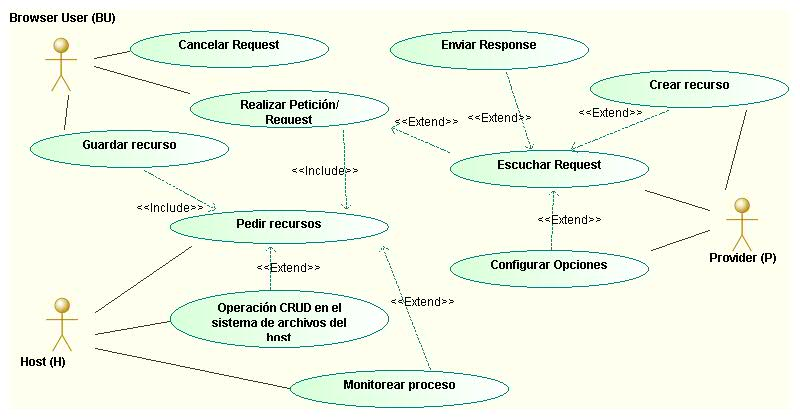
\includegraphics[scale=0.77]{figures/chap4/UCBrowser.jpg}
	        \caption{Diagrama de Caso de Uso del Web Browser.}
	        \label{fig:CUBrowser}
	    \end{figure}
	\end{landscape}


\section{Patrón Browser Infrastructure}
\label{chap4:BrokerPatt}
\subsection{Intent}
El patron Browser Infrastructure pattern permite la realización de la solicitud o \textit{request} de un recurso web en la Internet por parte de un BU, que es un usuario del Host que utiliza un navegador. El patrón permite visualizar la comunicación entre los componentes que conforman el browser así como la comunicación con el proveedor, al que se le realiza el \textit{request}.

\subsection{Ejemplo}
Dentro de un host es posible que exista una falta de recursos que necesite el usuario que lo opera. La solicitud de servicios o recursos externos es una de las razones de existir de la Internet. Esta operación es posible de realizarla de diferentes maneras, todo depende de lo que el Provider desea entregar.

\subsection{Contexto}
Browser User se encuentra al interior del Host y el Provider es accedido a través de Internet.  Es común que el contacto se da a través de aplicaciones Web, servers que se comunican a través del protocolo HTTP. Para poder visualizar los recursos que el BU puede necesitar y que el proveedor pueda quizás entregar, un navegador web permite completar tal labor de forma transparente al usuario.
\subsection{Problema}
Algunos BU puede que necesiten obtener recursos desde un Provider, pero el usuario puede que necesite utilizarlos en algún formato en especial o que sean presentados por pantalla para ser mejor visualizados. En este caso, si no se utiliza la herramienta adecuada puede que no sirva de mucho haber conseguido el recurso si no se puede ocupar correctamente. ¿Cómo pueden el Host y Provider estar preparados para esta situación?
La solución a este problema debe resolver las siguientes problemáticas:
\begin{itemize}
	\item Transparencia: el usuario detrás del Host no se debe preocupar de la maquinaria que existe mientras se realiza una petición a un Provider.
	\item Estabilidad: el Browser debe ser capaz de seguir funcionando, aún cuando una página haya tenido problemas para ser mostrada o exista un error.
	\item Aislación: cada \textit{request} realizada no debe interferir con las demás peticiones que se estén realizando.
	\item Heterogeneidad: Sin importar el tipo de Provider con el que se comunique, el Browser User debe poder comunicarse con cualquier tipo de Provider y también debe poder mostrar adecuadamente al usuario el recurso obtenido.
	\item Disponibilidad: El usuario del Host debe ser capaz de poder realizar peticiones en todo momento, sin perder fluidez.
\end{itemize}

\subsection{Solución}
Un Web Browser puede satisfacer las \textit{request} del user del Host a través de un Browser User, ya sea por una o varias instancias de Browser User, lo que permite tener una diversidad de opciones para navegar por sitios de Internet. Un Browser debe ser capaz de poder entregar una navegación rápida y estable, sin que cada sitio accedido afecte a los otros recursos adquiridos.
\subsection{Estructura}
El Browser Client (BC) es la entidad que representa el proceso principal de un Navegador Web y comprende la cantidad mínima de componentes que constituye un Web Browser. Un Host (H) que aloja e interactua con el BC, está compuesto por Hardware (HW) y un Sistema Operativo (SO). Al mismo tiempo, el Provider (P) posee también HW y SO, pero adicionalmente posee un Web Server (WS) que se encarga de recibir las peticiones externas. Browser Client, Sandbox, GPU Instance (GPUI) y Plugin son del tipo Process (Pr), que residen dentro de un Host (H) con un cierto tipo de sistema Operativo (OS). La mayoría de los navegadores existentes usan un componente central para realizar las operaciones que necesitan afectar al Host del Browser. La figura \ref{fig:BIPatt} muestra el diagrama del clases para el patrón Browser Infrastructure. Por cada recurso que un BC solicite, se crearán Sandbox (S) que alojarán una instancia del patrón Web Content Renderer el que permiten realizar la navegación y posterior visualización del recurso.
El componente BC actúa como un broker de las solicitudes de las Sandbox, lo que permite tener un control fino de los mensajes enviados, usando IPC/IPDL/COM, entre los procesos que se comunican. El GPU Instance y Plugins son elementos que pueden comunicarse directamente con el Sandbox, de esta manera cualquier necesidad de recursos del Host pasarán también por el Browser Client. 
Un usuario que desee hacer un \textit{request} de un recurso en Internet por medio de un navegador es lo que llamaremos Browser User (BU). Éste usa el Browser Client para realizar peticiones al Provider, donde éste último posiblemente utilice un Web Server para ese cometido (Figura \ref{fig:BIPatt})
	\begin{landscape}
	    \begin{figure}[h!t]
	        \centering
	        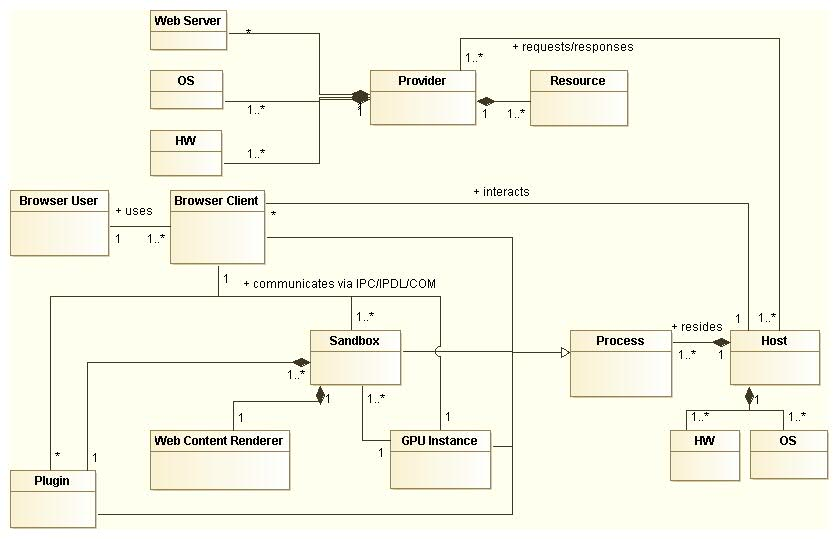
\includegraphics[scale=0.73]{figures/chap4/browserInfraPattern_v3.jpg}
	        \caption{Componentes de alto nivel del Browser.}
	        \label{fig:BIPatt}
	    \end{figure}
	\end{landscape}

\subsection{Dinámica}
Los casos de uso relacionados al patrón son los siguientes:
\begin{itemize}
	\item Realizar request (actor: Browser User)
	\item Cancelar request (actor: Browser User)
	\item Guardar recurso (actor: Browser User)
	\item Recibir Request (actor: Provider)
	\item Pedir recursos (actor: Host)
\end{itemize}
Detallaremos el caso de uso Realizar Request (Figura \ref{fig:SecReq}):
\subsubsection{Sumario} Un Browser User requiere de abrir un recurso URL que puede ser obtenido mediante el uso del protocolo HTTP, según los requerimientos del Provider. El Browser Client será usado por un Browser User para poder realizar la visualización del recurso URL.
\subsubsection{Actor} Browser User
\subsubsection{Precondiciones} El Host debe tener uno o más Browser Client para el usuario del Host. Además de estar conectado a una red o Internet. El Provider al que se desea contactar también debe estar disponible.
\subsubsection{Descripción}
Nota: Los mensajes entre el Browser Client y el Sandbox pueden ser tanto síncronos como asíncronos \cite{firefoxIPC,GCIPC}. No especificaremos en gran detalle , pues lo que importa en este trabajo será el origen y destino de los mensajes (no está dentro del ámbito ver la sincronización).
	\begin{enumerate}
		\item Un Browser User requiere acceder a una URL para obtener cierto recurso de un Provider, para esto usa un Browser Client ya instanciado por el Host. En el interior del Sandbox existe una instancia del patrón Web Content Renderer. 
		\item El Sandbox requiere los recursos del Host para obtener lo que hay detrás de la URL. Una petición es realizada desde el Sandbox al Browser Client a través de un canal de comunicación como: IPC, IPDL o COM (dependiendo el tipo de Browser usado), usando la API limitada que posee para comunicarse a un proceso de mayor privilegio. 
		\item El Browser Client recibe la solicitud, verifica a través de su motor de políticas/normas si la acción del Sandbox puede ser permitida.
		\item Si es permitada la acción del Sandbox, se utilizará la Network API que contiene el Browser Client para obtener recursos del Host (a través de llamadas al sistema). El Browser Client se comunica internamente con el Host, y este último debe revisar sus políticas y asegurarse que el Browser Client posee el privilegio de hacer la petición del recurso del Host.
		\item Si se permite el acceso el recurso, el Browser Client podrá realizar un \textit{request} a través de la Network API. Si el \textit{request} no es del tipo \textit{pre-flight}, el Provider recibirá el \textit{request} y trabajará sobre la petición.
		\item El Provider enviará un \textit{response} al \textit{request} enviado. Dependiendo como esté implementado el Browser Client, éste podría o no tener que esperar a la respuesta (síncrono o asíncrono) del Provider.
		\item Una vez obtenida la respuesta ésta es almacenada en cache, salvo que indique de no hacerlo.
		\item La respuesta del \textit{request} es enviada por el canal de comunicación al Sandbox del que se originó y posteriormente al Web Content Renderer. Si fue recibida una respuesta por parte de la \textit{request}, el Web Content Renderer está listo para preparar el parsing de la página web o utiliza un plugin o GPU para apoyar la visualización del recurso obtenido por la URL. En caso contrario el Web Content Renderer dentro del Sandbox creará una página de error.
		\item El \textit{Renderer} obtiene un bitmap que debe enviar al Browser Client, para que el Host pueda mostrarlo visualmente. Antes de realizarlo, debe revisar que el Sandbox que contiene el Web Content Renderer posea los permisos.
		\item Si los permisos son suficientes, el Browser Client envía el bitmap como parámetro en la llamada al sistema realizada al Host. Finalmente, el Host debe revisar que la llamada al sistema que realizó el Browser Client, tenga los permisos necesarios; de poseerlos, el bitmap se mostrará al Browser User por pantalla.
	\end{enumerate}
\subsubsection{Curso Alternativo} 
\begin{itemize}
\item El Provider no esté disponible.
\item El recurso al que apunta la URL no exista.
\item Se cancela el \textit{request} realizado.
	\end{itemize}
\subsubsection{Condiciones póstumas} El Browser recibe el recurso indicado por la URL y se muestra por el perísférico la salida del recurso al usuario del Host.
	\begin{landscape}
	    \begin{figure}[h!t]
	        \centering
	        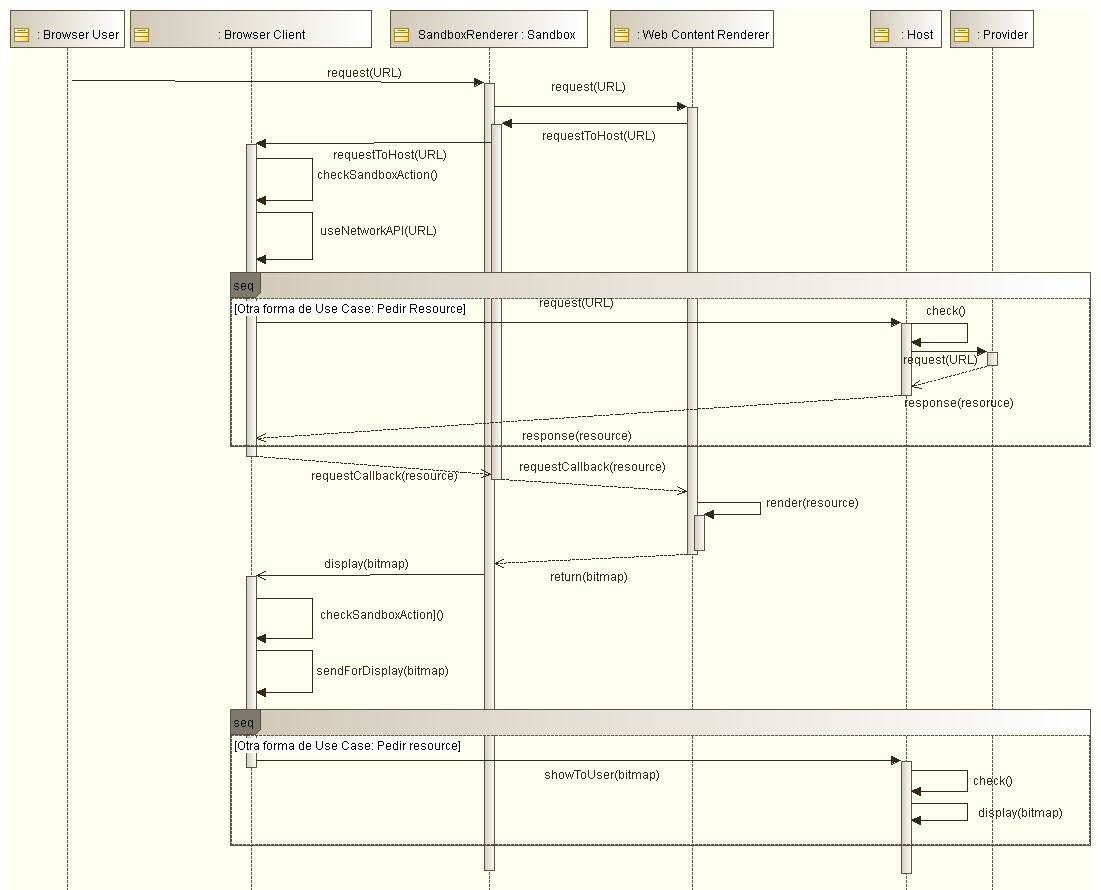
\includegraphics[scale=0.61]{figures/chap4/requestResource_v2.jpg}
	        \caption{Diagrama de Secuencia: Realizar Request.}
	        \label{fig:SecReq}
	    \end{figure}
	\end{landscape}
\subsection{Implementación}
\begin{itemize}
\item El Sandbox puede ser implementado de diversas maneras. Google Chrome \cite{sandboxGC} se basa en no reinventar la rueda y utiliza los mecanismos de protección que el Sistema Operativo (por ejemplo: Windows o Linux) del Host ya tiene incorporados para proteger al usuario, evitando que el proceso no tenga acceso al sistema de archivos y teniendo una API de llamadas al sistema muy restrictivas en el Web Content Renderer. Google Chrome, Firefox e Internet Explorer asumen que los Sandoboxs son procesos que deben regirse bajo el principio de menor privilegio (least privilege). La mínima configuración del Sandbox se compone de 2 procesos: El proceso privilegiado o Broker que es representado por el Browser Client, y el o los procesos que están bajo el Sandbox o targets.
\item Para hacer cumplir con el Same Origin Policy, Google Chrome, Firefox e Internet Explorer utilizan diferentes esquemas; por ejemplo: Google Chrome deja el trabajo a su Renderer (Web Content Renderer en este caso) para dejar aisladas las páginas/recursos de diversos sitios.
\end{itemize}
\subsection{Consecuencias}
El patrón Browser Infrastructure provee los siguientes beneficios:
\begin{itemize}
	\item Transparencia: La navegación del usuario se realizará casi de manera automática, solo en casos muy puntuales el usuario tendrá que tomar una decisión sobre el recurso que desea pedir.
	\item Estabilidad: Gracias a que el Browser Client, Sandbox, Plugin y GPU Instance son procesos del Host independientes, el fallo de uno no generará problemas en el otro (crash, corrupción de memoria, etc).
	\item Aislación: Dependiendo del tipo de aislación es posible separar los distintas peticiones, de manera que no interfieran entre sí, a menos que se desee.
	\item Heterogeneidad: Dado que cada Browser Client trata de seguir los estándares de la W3C, toda página que también siga éstas guías podrá ser visualizada, así como también otro tipo de recursos.
	\item Disponibilidad: Cada proceso es independiente y posee sus propias hebras de ejecución, y fueron creadas específicamente para que la interfaz de usuario pueda mantenerse fluida.
\end{itemize}
Al mismo tiempo, el patrón posee las siguientes debilidades:
\begin{itemize}
	\item Dado que se inician procesos independientes para navegar a un recurso (dependiendo el esquema que utilice el browser), es posible que una gran cantidad de recursos se vayan a usar para mantener todo abierto.
	\item Aquellos Provider que no hayan cumplido con las especificaciones de la W3C, mostrarán su resource de forma incorrecta por el Web Browser.
\end{itemize}
\subsection{Usos Comúnes}
\begin{itemize}
	\item Actualmente, la separación de los componentes del Browser en varios procesos, con diferentes niveles de acceso, se conoce como una Arquitectura Modular \cite{Vrbanec2013}. Esto permite la separación de preocupaciones del Navegador, lo que se traduce en una mayor estabilidad, aislación, seguridad y rapidez.
	\item Google Chrome se basa en la arquitectura modular, donde cada proceso Renderer se comunica con el Browser Kernel \cite{multiProcGC}. Internet Explorer, por ser privativo no da mucha información sobre su estructura o detalles de su implementación; \cite{Crowley2010} sobre la arquitectura Loosely-Coupled \cite{IE8-LCIE} y sus componentes, pero sin entrar tanto en detalle. Firefox, por su parte posee las dos implementaciones: monoprocesos y multiproceso. Electrolysis es el nombre de la arquitectura modular que se está implementado, pero que aún no ha sido finalizada completamente.
\end{itemize}
\subsection{Ejemplo Resuelto}
Con el patrón entregado ahora es posible poder navegar de forma fluida a todos los recursos en la Internet que deseamos. Es posible proveer a través de la aislación de los componentes: rapidez, seguridad y estabilidad. El Browser User solamente se molestará en la navegación, cuando se requiera de su autorización para ingresar a ciertos recursos del Host que sean privilegiados, como el sistema de archivos. Cada usuario del Host, puede utilizar el Browser Client que desee, dado que cada uno de ellos es aislado por procesos independientes, así también los otros Browser Clients entre si.


\subsection{Patrones Asociados}
\begin{itemize}
	\item El patrón Web Content Renderer, el cuál está en proceso de desarrollo, representa el subsistema dentro del Sandbox que permite realizar el parsing del \textit{resource} o recurso obtenido por medio de una petición.
	\item El patrón Browser--, también en desarrollo, representa el subsistema que representa el Navegador Web. Este componente actua como un Reference Monitor \cite{fernandez2013security} para todas las solicitudes que el Renderer llegara a necesitar.
	\item El Sandbox se comunica con el Browser Client siguiendo un patrón como el que indica el Policy Authorization \cite{fernandez2013security}. Por cada petición del Renderer, el Sandbox tendrá el acceso si las políticas que el Browser Client permiten tal acción.
\end{itemize}

\newpage
\chapter{Patrones de Mal Uso}
\label{chap6:Misuse}


\section{Identificando Amenazas y Patrones de Mal Uso}
En este capítulo presentaremos el análisis e identificación de las amenazas dentro del patrón presentado en el capítulo anterior, y 2 patrones de mal uso. Estos artefactos servirán de ejemplo de cómo usar la Arquitectura de Referencia obtenida. El objetivo de éste capítulo es conocer y visualizar los mal usos del sistema, en este caso del Browser, para poder educar a los desarrolladores de proyectos que basan sus sistemas en el uso de éste.
Este capítulo realiza los siguientes ítems: Un análisis de amenazas realizado sobre las actividades relacionadas en el caso de uso \textbf{Realizar Request} y \textbf{Recibir Request}, luego a partir del resultado del análisis se aplica la metodología explicada en el trabajo de [Bra08] para obtener una lista de amenazas. A través del listado de amenazas es posible detectar o inferir actividades de mal uso que pueden aparecer en uno o más casos de uso, que podrían resultar en una vulneración del sistema. Se presentarán los mal usos de actividades a través de patrones. Se han identificado 2 patrones y serán presentados a continuación.

\section{Identificando amenazas}
La identificación de amenazas es base para poder tomar medidas adecuadas para poder evitarlas. A través de la metodología de \cite{braz2008eliciting} es posible detectar y enumerar las amenazas de manera sistemática, al considerar cada actividad en cada caso de uso. Para enumerar las amenazas los diagramas de actividad ayudan en esta tarea.
Usando los casos de uso listado en el capítulo anterior, es posible revelar una lista de amenazas extensas. Solo para sintetizar el proceso, se usará un caso de uso y de éste se extraerá un patrón de mal uso.
La figura \ref{fig:ActDiagr} describe el diagrama de actividad compuesto, que involucra los casos de uso \textbf{Realizar Request} y \textbf{Recibir Request}. Varias amenazas pueden ser reveladas a través de las interacciones visualizadas en el diagrama, por ejemplo: Cuando se realiza la petición al servidor del recurso especificado por la URL, y se entrega otro recurso que no es el pedido. 

\begin{figure}[h!t]
    \centering
    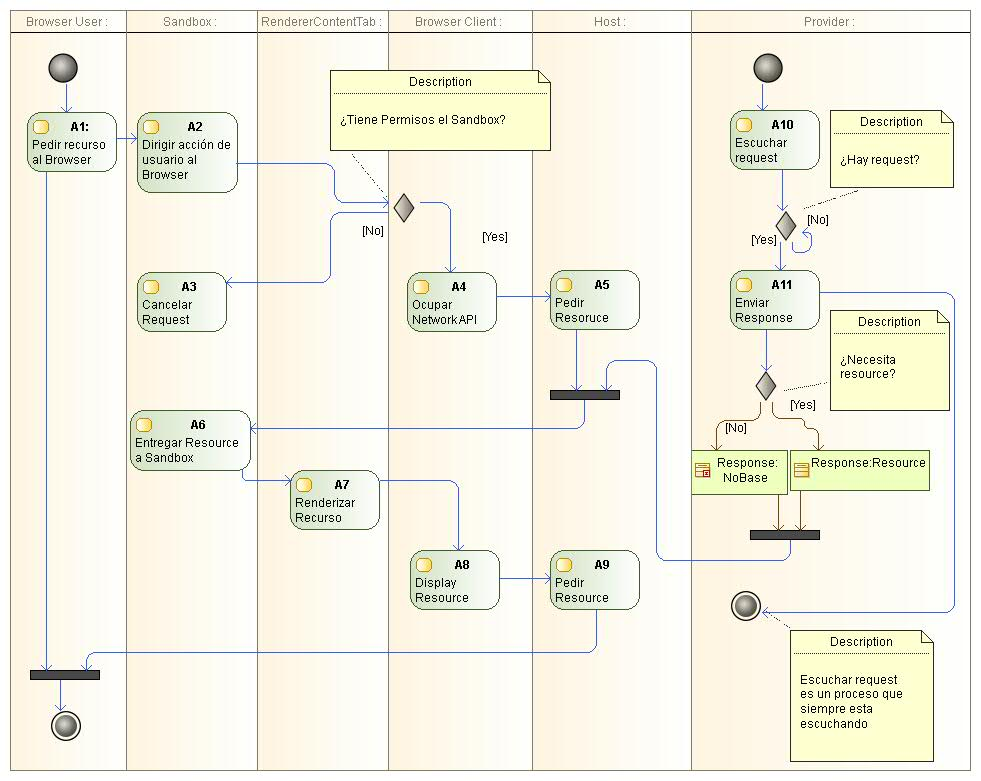
\includegraphics[scale=0.45]{figures/chap5/activityDiag_2.jpg}
    \caption{Diagrama de Actividad Compuesto para los casos de uso \textbf{Realizar Request} y \textbf{Recibir Request}.}
    \label{fig:ActDiagr}
\end{figure}

\begin{landscape}% Landscape page
\begin{table}[h!t]
\caption{Tabla con amenazas.}
\centering
\begin{tabular}{ |m{3.5em}|m{2.5em}|m{1.5em}|m{6em}|m{6em}|m{10em}|m{6em}|m{7em}|} 
\hline
Actor & Acción & ID & Sec. Attrib (CO/IN/AV/ACC) & Source (AIn/UIn/Out) & Descripción & Attacker & Asset\\
\hline
\multirow{5}{1em}{Browser User} & \multirow{5}{1em}{A1} & 1.1 & CO/IN & Out & Modificación de Tráfico/paquetes & Externo & Browser Client, Host\\ 
& & 1.2 & IN/CO & UIn/Out/In & Pedir recurso dentro del Host & Externo & Browser Client, Host\\
& & 1.3 & CO/IN/AV & UIn/Out & Contactar un Provider Malicioso & Externo & Browser Client, Host\\
& & 1.4 & CO & Out/UIn & Predecir comportamiento o análisis de tráfico & Externo, Process malicioso & Browser Client\\
& & 1.5 & CO/IN/ACC & Out & Conseguir contraseñas o información personal & Externo & Browser Client, Host\\
\hline
\multirow{4}{1em}{Host} & \multirow{5}{1em}{A5 y A9} & 5.1 & CO & Ain/UIn/Out & Divulgar información & Externo & Browser Client, Host\\ 
& & 5.2 & IN/CO & AIn/Out & Imitar a un Host honesto & Administrador Malicioso de Host & Browser Client, Provider\\
& & 5.3 & CO/IN/AV & Ain/Out/UIn & Contactar Provider Malicioso & Externo & Browser Client, Host\\
& & 5.4 & AV & Out & Impedir navegación & Externo & Browser Client\\
\hline
\multirow{2}{1em}{Provider} & \multirow{5}{1em}{A10} & 10.1 & IN/AV/ACC & Out & Aceptar request de cliente comprometido & Administrador Malicioso, Externo & Provider\\ 
& & 10.2 & CO & Ain/Out/UIn & Divulgar información & Externo & Provider\\

\hline
\end{tabular}
\label{tab:threats}
\end{table}
\end{landscape}

Hemos identificado algunas amenazas al analizar el curso de los eventos de los casos de uso: \textbf{Realizar Request} y \textbf{Recibir Request} (Figura \ref{fig:ActDiagr}). La tabla \ref{tab:threats} hace un sumario del análisis de cada acción en el diagrama de actividad, teniendo en cuenta los atributos de seguridad que podrían ser comprometidos, el origen de la amenaza y los recursos que pueden peligrar. Los atributos de seguridad principales son: Confidencialidad (CO), Integridad (IN), Disponibilidad (AV) y Responsabilidad (AC). El origen de la amenaza puede ser: actor autorizado (Ain), un actor no autorizado (UIn) o un externo (Out).
%Listar las amenazas que pueden ocurrir en el sistema no es suficiente para entender como los ataques ocurren. Es por esto que utilizaremos 2 patrones de mal uso, que permitirán describir como un ataque ocurre desde el punto de vista del atacante.

\section{Template de Patrones de Mal Uso}
\label{chap5:TemplateMP}
Esta sección describe cada parte del \textit{template} a usar para un Patron de Mal uso o Uso Indebido.

\subsection*{Nombre}
El nombre del patrón debe corresponder al nombre genérico dado al tipo específico de ataque en los repositorios estándares de ataques, como por el usado por el CERT \cite{cve}.

\subsection*{Intent o descripción básica}
Una descripción corta del propósito del patrón (qué problema resuelve para el atacante).

\subsection*{Contexto}
Describe el entorno genérico incluyendo las condiciones bajo a las cuales el ataque puede ocurrir. Esto puede incluir defensas mínimas presentes en el sistema, así como también vulnerabilidades típicas del sistema. El contexto puede ser especificado usando Diagramas de \textit{Deployment} de las partes relevantes del sistema así como también Diagaramas de Secuencia o de Colaboración que explayen el uso normal del sistema. Un diagrama de clases podría mostrar la estructura relevante del sistema. Se especifican además precondiciones para que el ataque ocurra.

\subsection*{Problema}
Desde la mirada del atacante, el problema es encontrar \textbf{cómo} atacar el sistema. Un problema adicional es cuando el sistema está protegido por mecanismos de defensa. Las fuerzas indican qué factores pueden ser requeridos en orden de ejecutar el ataque y en cómo realizarlo; por ejemplo, qué vulnerabilidades pueden ser explotadas. Además, qué factores podrían evitar que el ataque se pueda llevar acabo o lo retrasen.

\subsection*{Solución}
Esta sección describe la solución que resuelve el problema del atacante, ej: cómo el ataque puede alcanzar sus objetivos y los resultados esperados de éste. Diagramas en UML muestran los componentes del sistema involucrados. Diagramas de Secuencia o Colaboración muestran el intercambio de mensajes necesarios para cumplir con el ataque. Diagramas de actividad pueden añadir más detalle.

\subsection*{Componentes del sistema afectados (Dónde buscar evidencia)}
Esta sección adicional al \textit{template} original de un Patrón de Seguridad \cite{fernandez2013security} es nueva, dado que tiene relación con el mal uso realizado. La solución debe representar todos los componentes que están involucrados en el ataque, pero no debe ser una extensa lista, solo los más importantes para prevenirlo o lo escencial para una examinación forense. Esto puede ser representado por un diagrama de clases, que puede ser un subset o un superset del diagrama del contexto.

\subsection*{Usos comúnes}
Es prefeerido indicar los incidentes específicos en donde el ataque ha ocurrido. Pero en el caso de vulnerabilidades nuevas, donde el ataque aún puede que aún no se haya realizado, un contexto específico dónde el ataque pueda llevarse acabo es suficiente.

\subsection*{Consecuencias}
Discute los beneficios y desventajas del patrón de mal uso o uso indebido desde el punto de vista del atacante. ¿Es acaso el esfuerzo y costo gastado comparable a los resultados obtenidos? Esta es una evaluación que debe ser realizada por el atacante al decidir realizar el ataque; Diseñadores deben evaluar el riesgo de sus activos usando alpún enfoque de análisis de riesgos. La enumeración incluye buenos y malos aspectos, que deben ser emparejados a las fuerzas o \textit{forces}


\subsection*{Contramedidas y Evidencia Forense}
Esta sección describe las medidas de seguridad necesarias para detener, mitigar, o rastrear este tipo de ataque. Esto implica la enumeración de los Patrones de Seguridad o \textit{Security Patterns} que son efectivos contra este ataque. Desde un punto de vista Forense, se describe qué información puede ser obtenida en cada etapa rastreando el ataque y lo que puede ser deducido de los datos con el fin de identificar el ataque en específico. Finalmente, podría indicar qué información adicional debe ser recolectada en los componentes o unidades incolucrados para poder mejorar el análisis forense.

\subsection*{Patrones Similares}
Discute otros patrones de mal uso o uso indebido con diferentes objetivos pero realizados de manera similar, o con objetivos similares pero realizados de otra manera.

%PATRÓN

\section{Patrón de Mal Uso: Modificación de tráfico en el Web Browser}
En esta sección presentaremos un patrones de mal uso que describe la amenaza encontrada en el patrón Browser Infrastructure que hemos obtenido en este trabajo.
Una de las amenazas es que un atacante haya sido capaz de comprometer la respuesta obtenida desde el Provider contactado. El atacante podría tratar de reemplazar algunos parámetros de la respuesta del provider, entregando al Browser User un contenido distinto al original.

\subsection{Intent}
Un atacante podría cambiar contenido o dar uno diferente al esperado cuando el Web Browser (Browser User) recibe la response del Servidor o Provider. Realizando esta acción, el Navegador podría interpretar la información de una manera distinta a que si hubiera recibido el tráfico original.

\subsection{Contexto}
Un Navegador web obtiene resources desde un Provider para poder satisfacer un Browser User que lo necesita. Un Provider posee resources en forma de páginas web, servicios web u otro tipo. El Provider generalmente consiste en una Web App o Web server, que puede permitir entrada y salida de datos a otras aplicaciones, normalmente éstos están construidos usando HTML, Javascript y CCS. Sea que éste desea entregar servicios, como también otros deseen conectarse a él, todo tipo de comunicación estará encima del protocolo HTTP. Un Provider, dependiendo del tipo, puede llegar a recibir muchas peticiones de diversos Host para obtener recursos de éste. Dependiendo del tipo de peticiones, éstas pueden o no ser permitidas. Aquellas que son permitidas, el Provider generará una response a la \textit{request} del Host, la cuál terminará llegando de vuelta (o no) al Browser Client que generó el \textit{request}.

\subsection{Problema}
¿Cómo podría un atacante engañar al Browser User y Host, por medio de la modificación de tráfico entre las entidades participantes en la comunicación? Es posible que un atacante esté escondido entre medio de la comunicación que hay entre el Host y el Provider, lo que resulta en que el contenido modificado podría afectar dentro del RendererContentTab o el Browser Client. Esto en consecuencia podría traer diferentes resultados, desde el robo de información privada del Browser User que utiliza el Browser Client para personalizar la navegación como también los token de autenticación hacia los Providers que el Browser User ha utilizado previamente. Dependiendo del tipo de atacante, es posible que éste pueda incluso afectar al Host del Browser, dejando que el atacante pueda realizar actos maliciosos con los recursos del Host. 
El ataque puede sacar ventaja de las siguientes vulnerabilidades:
\begin{itemize}
	\item El \textbf{origen} u \textbf{origin} que define el Same Origin Policy que hace cumplir el Browser difiere en cada tipo de Web Browser \cite{W3C-SOP,Reis2009, Jackson2008, Crowley2010, Paola2006}.
	\item El \textbf{origin} no es suficiente como método de aislación entre resources (páginas web, scripts, css y otros) \cite{Silic2010, Barth2009, Yason, Liu2012}.
	\item Cualquiera puede crear una extensión o plugin, etc. para algún tipo de Browser y hacerlo pasar como algo inofensivo, pero el usuario no se daría cuenta que un ataque Man in the Browser podría estar ocurriendo \cite{Dougan2012,Utakrit2009,Liu2012,Barth2010}.  Éste programa, posiblemente malicioso, podría afectar el tráfico sin que queden rastros, pues tiene permisos del usuario al ser éste mismo quien autorizó su instalación.
	\item Es posible afectar al Browser Client, y en consecuencia al Host, sin tener que buscar vulnerabilidades en el Web Browser. Solamente utilizando métodos de ingeniería social, sobre el usuario del Host basta para lograr un ataque, pues es \textbf{el eslabón más débil}.
	\item La arquitectura para extender la funcionalidad del navegador, a través de extensiones, plugins y otros, depende demasiado del manufacturador. Y probablemente posee una gran superficie de ataque.
\end{itemize}

El ataque puede ser facilitado por:
\begin{itemize}
	\item Existen muchas herramientas para realizar ataques de ingeniería social, lo que permite hacer que el Browser User acepte realizar la instalación de extensiones o plugin maliciosos más fácilmente.
	\item Cualquier script basado en texto puede ser usado para explotar el intérprete del navegador web. Muchas veces también es posible utilizar los mismos elementos del lenguaje de scripting para poder pasar ciertas barreras de seguridad entregadas por el SOP, pues el lenguaje está basado en prototipos. 
	\item Los manufacturadores de Navegadores no poseen aún mecanismos de defensa que permitan identificar efectivamente cuando un recurso puede ser malicioso.
	\item Los métodos de cifrado no pueden hacer nada contra un ataque que puede modificar el tráfico antes de enviar o después de recibir el mensaje.
	\item No existen mecanismos de defensa estandarizados, pues cada manufacturador realiza lo necesario para la marca a la que se acopla. Si el Host posee muchos browser, la superficie de ataque es bastante mayor.
\end{itemize}
\subsection{Solución}
La solución estructural usada es la misma creada por el patrón Browser Infrastructure que se revisó en el capítulo 4. La clase Attacker es cualquier entidad que podría llevar a cabo una acción arriesgada contra la integridad del Browser, usuario, Host y Provider (Figura \ref{fig:BIMisuse}). El atacante es capaz tanto de interceptar las response que el Provider envía al Browser Client usando al Host como receptor, o haciendo que el Browser realice modificaciones en el input que va hacia el Provider, utilizando scripts u otro resources.
\begin{figure}[h!t]
	        \centering
	        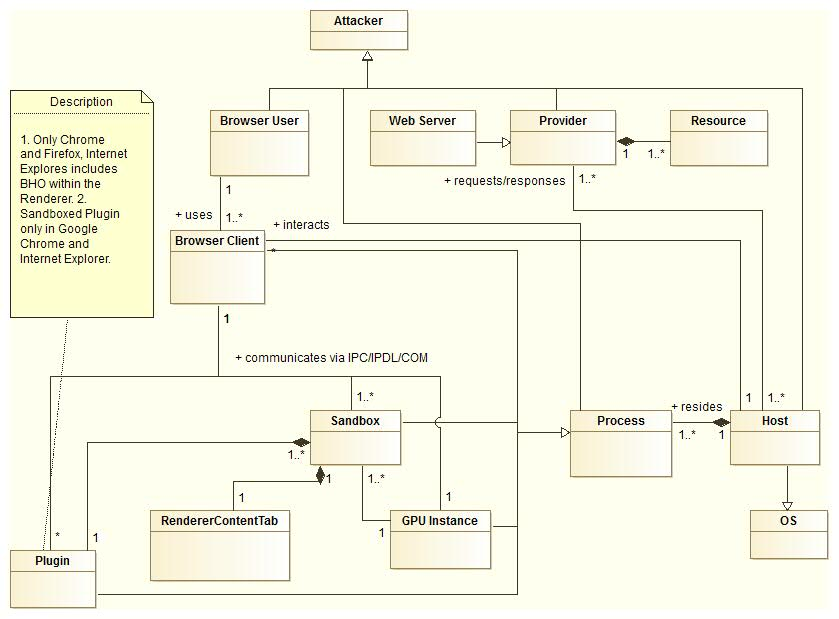
\includegraphics[scale=0.5]{figures/chap5/patronMisuse.jpg}
	        \caption{Diagrama de Clases para el patrón de Misuse.}
	        \label{fig:BIMisuse}
    \end{figure}

\subsection{Dinámica}
En la figura \ref{fig:SeqMisuse} se muestra la serie de pasos necesarios, para realizar uno de los tantos mal usos que se pueden realizar durante el caso de uso Realizar \textit{request}. El atacante queda entre el Browser Client y el Host, interceptando la realización del \textit{request} original y modificando el tráfico a su gusto; usualmente un ataque basado en este mal uso se le llama Man-in-the-Browser (MITB) \cite{Liu2012, Barth2010, Utakrit2009, Dougan2012}. Esto podría perfectamente suceder cuando el Browser User ha permitido la instalación de plugins, extensiones o programas externos en el Host y Browser Client.
\begin{figure}[h!t]
	        \centering
	        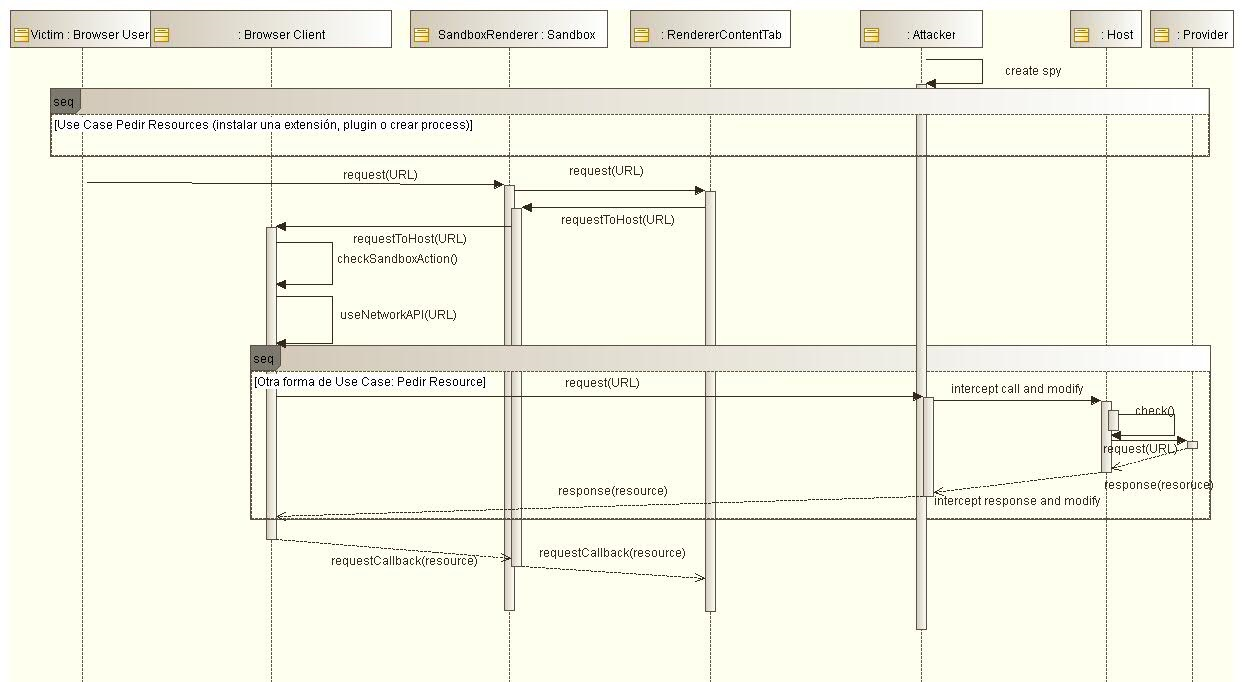
\includegraphics[scale=0.45]{figures/chap5/patronMisuseSeq.jpg}
	        \caption{Diagrama de Secuencia para el Mal uso: Modificación de tráfico en el Web Browser.}
	        \label{fig:SeqMisuse}
    \end{figure}
	
	\subsubsection{Sumario} El atacante intercepta el tráfico entre Host y Browser Client.
	\subsubsection{Actor} Atacante
	\subsubsection{Precondiciones} Para que el ataque pueda pasar desapercibido, es necesario que el Browser User o el usuario detrás del browser haya caído primero en un ataque de ingeniería social o el atacante haya podido instalar directamente un proceso o componente malicioso en el Host directamente.
	\subsubsection{Descripción}
			\begin{enumerate}
				\item Un atacante utiliza alguna técnica de ingeniería social o vulnerabilidad en el sistema, para crear una entidad que se encargará de estar entre medio del Browser Client y el Provider. Para esto realiza el caso de uso \textbf{Pedir Resources} para que el proceso, plugin o extensión se aloje en el Host.
				\item Un Browser Consumer desea hacer un \textit{request} a cierta URL, por lo que los primeros pasos de \textbf{Realizar Request} son similares.
				\item En el momento en que el Browser Client va a realizar la llamada al sistema para enviar el mensaje del Host al Provider, el Browser Client llamará al plugin, extensión o process malicioso, pues el Browser Client ha sido intervenido para que realice esa acción de este modo.
				\item El atacante entonces recibirá todo el tráfico del Browser Client, el cuál podría modificar a su antojo.
				\item Finalmente la víctima está totalmente comprometida.
			\end{enumerate}
	\subsubsection{Post condiciones} La víctima quedará completamente comprometida y probablemente no sea posible detectar la alteración del mensaje, pues también es posible que se modifiquen los log del Host.
	\subsubsection{Usos Conocidos} El Web Browser es un software que posee diversas implementaciones, por lo tanto la cantidad de vectores de ataque es significativa. Algunos de éstos son:
			\begin{itemize}
				\item  Una extensión basada en la arquitectura de Chrome o la API WebExtension Firefox, podría interceptar los datos antes que llegue al Browser Client \cite{Paola2006} o dado a una vulnerabilidad del mismo elemento un atacante se está aprovechando de su funcionalidad para realizar ataques \cite{Liu2012, Barth2010}. Dado que el Plugin, la extensión o el process son elementos que el Host confía, es posible que el ataque sea indetectable y los métodos de cifrado no sirven como medida de mitigación.
				\item Éste tipo de ataque puede ser usado como base para otros ataques más avanzados. Un ejemplo es cuando el Browser posee vulnerabilidades \textit{cross-origin javascript capability leaks}, donde los diferentes modelos de seguridad usados por Javascript y el DOM pueden interferir entre sí, causando que una petición \textit{cross-origin} se pueda realizar aún cuando SOP debería ser capaz de detener tal ataque \cite{Barth2009}.
			\end{itemize}


\subsection{Consecuencias}
	El mal uso tiene las siguientes consecuencias para el Attacker:
	\begin{itemize}
		\item Objetivos: pueden ser diversos, destacándose el vandalismo, personificar a otra persona u obtener una ganancia monetaria. Mientras el atacante se pueda interponer entre el Host y el tráfico que se envía al Provider, la confidencialidad e integridad de los datos está completamente perdida. La privacidad del usuario ya no se puede asegurar tampoco.
		\item Silencioso: Dado que el atacante ha logrado interponerse entre las llamadas de sistema que se realizan al Host para enviar los datos al Provider, el Host no reconocerá ni logueará ninguna anomalía. Las llamadas hechas al Host son totalmente legales y nada fuera de lo normal para éste.
		\item El atacante podría realizar acciones que afecten la integridad del Host.
	\end{itemize}
	Posibles fuentes de fallo:
	\begin{itemize}
		\item Si el Browser User es capaz de evitar o ignorar el ataque de Ingeniería Social realizado al comienzo, no existiría este mal uso. Esto debe considerar que el usuario también no se encuentre con páginas o contenido malicioso, que podrían afectar otro componente de Browser, pero que causarían en el mismo efecto del Mal Uso señalado.
	\end{itemize}

\subsection{Contramedidas} 
	Para prevenir este tipo de mal uso se recomienda tomar las siguientes medidas preventivas:
	\begin{itemize}
		\item Servicios de Reputación como Smart Screen de Internet Explorer y Download Application de Google Chrome, ayudan a identificar páginas y contenido/resources que podrían contener malware que se instale como plugins, entensiones o process en el Host del Browser User.
		\item Entregando educación sobre los peligros de navegar por Internet y aclarar al usuario que él es la última línea de defensa contra éste tipo de ataques.
		\item White y Black list instaladas en los browser son una medida preventiva para evitar la navegación en páginas o recursos maliciosos ya conocidos.
		\item Navegadores como Google Chrome e Internet Explorer ofrecen el Sandboxing. Éste mecanismo de defensa limita las acciones del atacante, que pudieran afectar la integridad del sistema.
	\end{itemize}

\subsection{Evidencia Forense}
	¿Dónde es posible encontrar evidencia?
	Dependiendo de lo deseado por el atacante, las acciones que cometerá pueden diferir. Sin embargo el log interno del browser debería de poder servir para auditar el sistema, esto gracias a que mientras no se haya encontrado una vulnerabilidad en el Sandbox del Browser, el atacante no puede borrar completamente sus huellas.

\subsection{Patrones relacionados}
	\begin{itemize}
		\item En el patrón Browser Infrastructure, el Browser Client actúa como el Reference Monitor explicado en \cite{fernandez2001pattern}.
	\end{itemize}

\newpage
%\input{chapters/conclusion.tex}

%\backmatter
%\addcontentsline{toc}{chapter}{References}
\bibliography{refTodas}
\bibliographystyle{IEEEtran}

\appendix
%\input{chapters/anexos.tex}
%\input{chapters/anexo2.tex}
\end{document}